% This one will format for two-sided binding (ie left and right pages have mirror margins; blank pages inserted where needed):
\documentclass[a4paper,twoside]{ociamthesis}
% This one will format for one-sided binding (ie left margin > right margin; no extra blank pages):
%\documentclass[a4paper]{ociamthesis}
% This one will format for PDF output (ie equal margins, no extra blank pages):
%\documentclass[a4paper,nobind]{ociamthesis} 

% !TEX root = ../main.tex

%%%%% SELECT YOUR DRAFT OPTIONS
% Three options going on here; use in any combination.  But remember to turn the first two off before
% generating a PDF to send to the printer!
% This highlights (in blue) corrections marked with (for words) \mccorrect{blah} or (for whole
% paragraphs) \begin{mccorrection} . . . \end{mccorrection}.  This can be useful for sending a PDF of
% your corrected thesis to your examiners for review.  Turn it off, and the blue disappears.
\correctionstrue

%%%%% BIBLIOGRAPHY SETUP
\usepackage{natbib}
\bibliographystyle{plainnat}
% This makes the bibliography left-aligned (not 'justified') and slightly smaller font.
\renewcommand*{\bibfont}{\small}
\setlength{\bibsep}{1pt}
\setcitestyle{square}

%%%%% THESIS / TITLE PAGE INFORMATION
% Everybody needs to complete the following:
\title{\vspace{20pt}Neural Networks for Inference,\\ Inference for Neural Networks}
\author{Stefan Webb}
\college{Wadham College}

% Your full degree name.  (But remember that DPhils aren't "in" anything.  They're just DPhils.)
\degree{Doctor of Philosophy}
% Term and year of submission, or date if your board requires (eg most masters)
\degreedate{Michaelmas 2018}

\usepackage{microtype}

% use Times
\usepackage{times}
% For figures
\usepackage{graphicx} % more modern
%\usepackage{epsfig} % less modern
%\usepackage{subfigure} 
\usepackage{subcaption} 
%\graphicspath{{./part/ipmcmc/figures/}{./misc/figures/}{./bopp/figures/}{./opt/figures/}{./design/figures/}{./nest/figures/}{./inf/figures/}{./part/figures/}{./bayes/figures/}{./probprog/figures/}{./part/figures/}}
\usepackage{tikz}
\usetikzlibrary{fit}					% fitting shapes to coordinates
\usetikzlibrary{backgrounds}	% drawing the background after the foreground
\usepackage{setspace}
\usepackage{pdfpages}

\usepackage{cancel}

%\usepackage{svg}

% For algorithms


% For math
\usepackage{amsthm}
\usepackage{dsfont}
\usepackage{amssymb,amsmath}
\usepackage{bbm}

%\newcommand{\theHalgorithm}{\arabic{algorithm}}

\usepackage{hyperref}

\usepackage{bibentry}
\nobibliography*


% % BOPP

%\usepackage{enumitem}
%\setlist[itemize]{leftmargin=*}
%\usepackage{paralist}
\usepackage{footmisc}
\usepackage{listings}
\usepackage{color}
\usepackage{xcolor}
\usepackage{textcomp}
\usepackage{xspace}
\usepackage{amsbsy}
\usepackage{siunitx}
%\usepackage{algorithmicx}
%\usepackage{algpseudocode}
\usepackage{mathtools}
\usepackage{array}
\usepackage{booktabs}
\usepackage{adjustbox}
\usepackage{microtype}
\usepackage{todonotes}

\usepackage{wrapfig}
\usepackage{thmtools}
\usepackage{thm-restate}

%\newcommand{\angurl}{\scriptsize \url{http://www.robots.ox.ac.uk/~fwood/anglican}}
%\newcommand{\myurl}{\scriptsize \url{https://bitbucket.org/twgr/ipmcmc}}

\definecolor{darkgreenClj}{rgb}{0.25,.5,0.25}
\definecolor{blueClj}{rgb}{0,0.33,0.66}
\definecolor{redClj}{rgb}{0.66,0.0,0.0}
\definecolor{purpleClj}{rgb}{0.33,0,0.66}
\definecolor{cyanClj}{rgb}{0.0,0.5,0.5}
\definecolor{orangeClj}{rgb}{0.75,0.35,0.0}
\definecolor{grayClj}{rgb}{0.4,0.4,0.4}
\lstset{ 
	language=Lisp, 
	basicstyle=\small\ttfamily,
	keywordstyle={}, 
	alsoletter={<-,->,:,*,/,?,+,-,/,>,<,=, &},
	commentstyle=\em \color{gray}, 
	frame=lines,
	%float=tbph,
	% captionpos=b,
	showstringspaces=false, 
	keywordstyle=[1]\bf\ttfamily\color{blueClj},
	keywords=[1]{BO,theta-best,bo-acquire,sample-initial-points,sample,observe,observe<-,predict,mem,store,retrieve,return,catch,throw,absorb,produce,with-primitive-procedures,conditional,result,log-marginal,mean,
		->sample,->observe,->result},
	keywordstyle=[2]\bf\ttfamily\color{redClj},
	keywords=[2]{if,let,letfn,loop,looppredict,recur,or,trampoline,assoc,argmax,count,cons,conj,
		do,first,fn,get,keys,lazy-seq,map,nth,mat/add,mat/div,print,reduce,repeat,repeatedly,rest,set,shape,take,vec,
		when,max,fn?,inc,sample*,observe*},
	keywordstyle=[3]\bf\ttfamily\color{cyanClj},
	keywords=[3]{dirichlet-discrete,exponential,flip,gamma,beta,mvn-niw,normal,uniform-continuous,distribution,factor,mvn,uniform,bernoulli,uniform-discrete,poisson,
		simulate,abc-likelihood,student-t,dirichlet},
	keywordstyle=[4]\bf\ttfamily\color{purpleClj},
	keywords=[4]{defopt,defquery,doopt,doquery,query,defdist,infer,checkpoint,exec,defm,cps-of-expression,
		defn,def,declare},
	keywordstyle=[5]\bf\ttfamily\color{orangeClj},
	keywords=[5]{:lmh,:ipmcmc,:war,:peace,:log-weight,:result,:id,:dist,:cont,:value,:state,:importance,:smc,:pgibbs},
	mathescape=true,
	stringstyle={},
		keywordstyle=[6]\bf\ttfamily\color{darkgreenClj},
		keywords=[6]{+,-,nil,>,<,*,/,=, &,->>,->,true,false},
		mathescape=true,
		stringstyle={},
} 
\lstnewenvironment{code}[2]{\lstset{caption=#1,label=#2}}{}

\newtheorem{example}{Example} 
\newtheorem{theorem}{Theorem}[chapter]
\newtheorem{lemma}[theorem]{Lemma} 
%\newtheorem{proposition}[proposition]{Proposition} 
\newtheorem{remark}{Remark}[chapter]
%\newtheorem{corollary}[corollary]{Corollary}
\newtheorem{definition}{Definition}[chapter]
%\newtheorem{conjecture}[conjecture]{Conjecture}
%\newtheorem{axiom}[axiom]{Axiom}

% % % % % % % % % % % % % % % % % % %


\usepackage{naesseth}
%\usepackage{packages/algorithm,packages/algorithmic}
\usepackage{abbreviations}
\usepackage{tikz-bayesnet}

\usepackage{algorithmicx}
\usepackage[chapter]{algorithm}
\usepackage{algpseudocode}
\usepackage{setspace}
% % % % % % % % %
\algnewcommand\algorithmicswitch{\textbf{switch}}
\algnewcommand\algorithmiccase{\textbf{case}}
\algnewcommand\algorithmicassert{\texttt{assert}}
\algnewcommand\Assert[1]{\State \algorithmicassert(#1)}%
% New "environments"
\algdef{SE}[SWITCH]{Switch}{EndSwitch}[1]{\algorithmicswitch\ #1\ \algorithmicdo}{\algorithmicend\ \algorithmicswitch}%
\algdef{SE}[CASE]{Case}{EndCase}[1]{\algorithmiccase\ #1}{\algorithmicend\ \algorithmiccase}%
%\algtext*{EndSwitch}%
\algtext*{EndCase}%
\algnewcommand{\IIf}[1]{\State\algorithmicif\ #1\ \algorithmicthen}
\algnewcommand{\EndIIf}{\unskip\ \algorithmicend\ \algorithmicif}


%%%%%%%%%%%%%

\usepackage{titlesec}

\titlespacing*\section{0pt}{14pt plus 4pt minus 2pt}{3pt plus 2pt minus 2pt}
\titlespacing*\subsection{0pt}{10pt plus 4pt minus 2pt}{3pt plus 2pt minus 2pt}
\titlespacing*\subsubsection{0pt}{10pt plus 4pt minus 2pt}{3pt plus 2pt minus 2pt}

\setlength{\intextsep}{14pt}%
\setlength{\columnsep}{18pt}%

\DeclarePairedDelimiterX{\infdivx}[2]{\{}{\}}{%
  #1\;\delimsize\|\;#2%
}
\newcommand{\infdiv}{\text{KL}\infdivx}

\newcommand{\model}{$p_\phi(\mathbf{x},\mathbf{z})$}
\newcommand{\fixedmodel}{$p(\mathbf{x},\mathbf{z})$}
\newcommand{\guide}{$q_\psi(\mathbf{z}\mid\mathbf{z})$}
\newcommand{\logmodel}{\lg\left(\model\right)}
\newcommand{\logfixedmodel}{\lg\left(\model\right)}
\newcommand{\logguide}{\lg\left(\guide\right)}
\usepackage{breakcites}

%\ShortHeadings{Automating Inference, Learning, and Design}{Tom Rainforth}
%\firstpageno{1}

\begin{document} 

%%%%% CHOOSE YOUR LINE SPACING HERE
% This is the official option.  Use it for your submission copy and library copy:
%\setlength{\textbaselineskip}{22pt plus2pt}
\setlength{\textbaselineskip}{21pt plus2pt}
% This is closer spacing (about 1.5-spaced) that you might prefer for your personal copies:
%\setlength{\textbaselineskip}{18pt plus2pt minus1pt}

% You can set the spacing here for the roman-numbered pages (acknowledgements, table of contents, etc.)
\setlength{\frontmatterbaselineskip}{18pt plus1pt minus1pt}

% Leave this line alone; it gets things started for the real document.
\setlength{\baselineskip}{\textbaselineskip}

%\renewcommand{\contentsname}{\hfill Contents \hfill \hfillline}

%%%%% CHOOSE YOUR SECTION NUMBERING DEPTH HERE
% You have two choices.  First, how far down are sections numbered?  (Below that, they're named but
% don't get numbers.)  Second, what level of section appears in the table of contents?  These don't have
% to match: you can have numbered sections that don't show up in the ToC, or unnumbered sections that
% do.  Throughout, 0 = chapter; 1 = section; 2 = subsection; 3 = subsubsection, 4 = paragraph...

% The level that gets a number:
\setcounter{secnumdepth}{3}
% The level that shows up in the ToC:
\setcounter{tocdepth}{1}

% JEM: Pages are roman numbered from here, though page numbers are invisible until ToC.  This is in
% keeping with most typesetting conventions.
\begin{romanpages}
	
	% Title page is created here
	\maketitle
	
	%%%%% DEDICATION -- If you'd like one, un-comment the following.
	%\begin{dedication}
	%This thesis is dedicated to\\
	%someone\\
	%for some special reason\\
	%\end{dedication}
	
	
	%%%%% ABSTRACT -- Nothing to do here except comment out if you don't want it.
	\begin{abstract}
		\vspace{20pt}
Bayesian statistics is a powerful framework for modeling the world and reasoning over uncertainty. It provides a principled method for representing our prior knowledge, and updating that knowledge in the light of new information. Traditional Bayesian statistics, however, has been limited to simple models. Two of the main limiting factors for this are the expressiveness and flexibility of the probability distributions used, and the computational restrictions in performing inference and model learning. In this thesis, we consider how neural networks (NNs) can be used to assist with both of these problems. In particular, we will look at how NNs can assist in the inference process and how we can perform inference over flexible NN models.

NNs are helpful for Bayesian inference in generative models. They are useful for producing the flexible variational families required for successful variational inference (VI), as well as learning distributed representations of model variables for guiding the distributional relationships of the model. Inference, on the other hand, is useful for quantifying uncertainty in NN discriminative models. For instance, with ``Bayesian NNs'' one can use inference to learn a distribution over the NNs parameters and hence quantify our uncertainty over the model's predictions. However, this increased flexibility in modeling and inference comes with challenges in inference and representation.

We present three pieces of original work in this thesis towards solving these challenges. We produce an algorithm for constructing the factorization of variational approximations in an optimal way to improve the fidelity and scalability of VI. We develop a framework for distributed Bayesian learning that is particularly useful for large Bayesian NNs and is less prone to the stale gradient of non-Bayesian approaches. We finish by considering an example of how Bayesian inference can be applied to NNs in a non-standard context by reinterpreting the problem of estimating NN robustness as an inference problem.
	\end{abstract}
	
	%%%%% ACKNOWLEDGEMENTS -- Nothing to do here except comment out if you don't want it.
	\begin{acknowledgements}
		\vspace{20pt}
I would like to thank first and foremost my girlfriend, Anjuli, and my parents back in Australia. Without your love and support I could not have gotten through this arduous time. I would also like to extend a special thanks to Tom Rainforth, whose mentorship was instrumental in bringing our work to publication---you have taught me a lot. I am grateful to my supervisors, Pawan and Yee Whye, for their guidance and direction, and my colleagues and collaborators in Engineering Science and Statistics for providing a stimulating intellectual environment. Lastly, I am thankful to Steve Roberts and Niki Trigoni, and the financial support provided by the AIMS CDT program and the EPSRC, for providing the opportunity to study at Oxford and become a published researcher, all the while experiencing many wonderful things---music, theatre, debates, speeches, and meeting the love of my life.
	\end{acknowledgements}
	
	
	%%%%% MINI TABLES
	% This lays the groundwork for per-chapter, mini tables of contents.  Comment the following line
	% (and remove \minitoc from the chapter files) if you don't want this.  Un-comment either of the
	% next two lines if you want a per-chapter list of figures or tables.
	%\dominitoc % include a mini table of contents
	%\dominilof  % include a mini list of figures
	%\dominilot  % include a mini list of tables
	
	% This aligns the bottom of the text of each page.  It generally makes things look better.
	\flushbottom
	
	% This is where the whole-document ToC appears:
	\tableofcontents
	
	%\listoffigures
	%\mtcaddchapter
	% \mtcaddchapter is needed when adding a non-chapter (but chapter-like) entity to avoid confusing minitoc
	
	% Uncomment to generate a list of tables:
	%\listoftables
	%	\mtcaddchapter
	
	%%%%% LIST OF ABBREVIATIONS
	% This example includes a list of abbreviations.  Look at text/abbreviations.tex to see how that file is
	% formatted.  The template can handle any kind of list though, so this might be a good place for a
	% glossary, etc.
	%% THIS STYLE FILE CONTAINS SOME COMMON ABBREVIATIONS

\RequirePackage{xspace} % Used to get the \xspace command for spaces after abbreviations.
\newcommand\textabbr[1]{\mbox{#1}}

%%%%%%%%%%%%%%%%%%%%%%%%%%%%%%%%%%%%%%%%%%%%%%%%%%%%%%%%%%%%%%%%%%%%%
%                      STANDARD ABBREVIATIONS                       %
%%%%%%%%%%%%%%%%%%%%%%%%%%%%%%%%%%%%%%%%%%%%%%%%%%%%%%%%%%%%%%%%%%%%%

\newcommand{\eg}{e.g.\@\xspace}
\newcommand{\ie}{i.e.\@\xspace}
\newcommand{\etc}{etc}               % Used at the end of a sentence
\newcommand{\etcin}{etc.\@\xspace}   % Used in scentence
\newcommand{\wrt}{w.r.t.\@\xspace}
\newcommand{\sbto}{s.t.\@\xspace}
\newcommand{\cf}{cf.\@\xspace}
\newcommand{\vs}{vs.\@\xspace}
\newcommand{\NB}{N.B.\@\xspace}
\newcommand{\subto}{\text{s.t.} \:}

\newcommand{\io}{i.o.\@\xspace}
\newcommand{\asintext}{almost surely\@\xspace}
\newcommand{\allmosteverywhere}{a.e.\@\xspace}
\newcommand{\asend}{a.s}
\newcommand{\wpone}{w.p.1.\@\xspace}
\newcommand{\aeend}{a.e}

%%%%%%%%%%%%%%%%%%%%%%%%%%%%%%%%%%%%%%%%%%%%%%%%%%%%%%%%%%%%%%%%%%%%%
%                COMMON TOPIC SPECIFIC ABBREVIATIONS                %
%%%%%%%%%%%%%%%%%%%%%%%%%%%%%%%%%%%%%%%%%%%%%%%%%%%%%%%%%%%%%%%%%%%%%

% Models
\newcommand\ssm{SSM\@\xspace}      % State-space model
\newcommand\lgss{LGSS\@\xspace}    % Linear Gaussian state-space
\newcommand\pgm{PGM\@\xspace}    % Probabilistic graphical model
\newcommand\mrf{MRF\@\xspace}    % Markov Random field
% Methods
\newcommand\exm{EM\@\xspace}      % Expectation maximization
% Monte Carlo methods
\newcommand\is{IS\@\xspace}      % Importance Sampling
\newcommand\sis{SIS\@\xspace}      % Sequential Importance Sampling
\newcommand\stpf{ST-PF\@\xspace}   % Space-Time Particle Filter
\newcommand\smc{SMC\@\xspace}      % Sequential Monte Carlo
\newcommand\csmc{CSMC\@\xspace}      % Conditional Sequential Monte Carlo
\newcommand\nsmc{NSMC\@\xspace}      % Nested Sequential Monte Carlo
\newcommand\mcmc{MCMC\@\xspace}    % Markov chain Monte Carlo
\newcommand\pmcmc{PMCMC\@\xspace}  % Particle MCMC
\newcommand\ipmc{iPMCMC\@\xspace}    % interacting Particle Markov Chain Monte Carlo
\newcommand\ipmcmc{iPMCMC\@\xspace}    % interacting Particle Markov Chain Monte Carlo
\newcommand\pmmh{PMMH\@\xspace}    % Particle Marginal Metropolis-Hastings
\newcommand\pg{PG\@\xspace}        % Particle Gibbs
\newcommand\apf{APF\@\xspace}        % Auxiliary particle filter
\newcommand\ess{ESS\@\xspace}	   % Effective Samples Size
\newcommand\ers{ERS\@\xspace}	   % Effective Resample Size

\newcommand\hone{H1\@\xspace}	
\newcommand\htwo{H2\@\xspace}	

\DeclareRobustCommand*\matlab{\mbox{Matlab}\xspace}

%%%%%%%%%%%%%%%%%%%%%%%%%%%%%%%%%%%%%%%%%%%%%%%%%%%%%%%%%%%%%%%%%%%%%
			%                iPMCMC              %
%%%%%%%%%%%%%%%%%%%%%%%%%%%%%%%%%%%%%%%%%%%%%%%%%%%%%%%%%%%%%%%%%%%%%

\newcommand\nw{\bar w} % Normalised weights
\newcommand\nz{\zeta} % Normalised conditional sampling weights

%%%%%%%%%%%%%%%%%%%%%%%%%%%%%%%%%%%%%%%%%%%%%%%%%%%%%%%%%%%%%%%%%%%%%
			%                BOPP               %
%%%%%%%%%%%%%%%%%%%%%%%%%%%%%%%%%%%%%%%%%%%%%%%%%%%%%%%%%%%%%%%%%%%%%

\newcommand{\lsi}[1]{\lstinline$#1$}

\newcommand{\sample}{\lstinline$sample$\xspace}
\newcommand{\observe}{\lstinline$observe$\xspace}
\newcommand{\observes}{\lstinline$observe<-$\xspace}
\newcommand{\predict}{\lstinline$predict$\xspace}
\newcommand{\simulatec}{\lstinline$simulate$\xspace}
\newcommand{\abcl}{\lstinline$abc-likelihood$\xspace}
\newcommand{\boppfactor}{\lstinline$factor$\xspace}

\newcommand{\samplecps}{\lstinline$->sample$\xspace}
\newcommand{\observecps}{\lstinline$->observe$\xspace}

\newcommand{\checkpoint}{\lstinline$checkpoint$\xspace}
\newcommand{\anginfer}{\lstinline$infer$\xspace}

\newcommand{\defdist}{\lstinline$defdist$\xspace}
\newcommand{\defquery}{\lstinline$defquery$\xspace}
\newcommand{\query}{\lstinline$query$\xspace}
\newcommand{\defopt}{\lstinline$defopt$\xspace}
\newcommand{\doquery}{\lstinline$doquery$\xspace}
\newcommand{\doopt}{\lstinline$doopt$\xspace}
\newcommand{\defn}{\lstinline$defn$\xspace}
\newcommand{\defm}{\lstinline$defm$\xspace}
\newcommand{\normal}{\lstinline$normal$\xspace}
\newcommand{\studentt}{\lstinline$student-t$\xspace}
\newcommand{\betaa}{\lstinline$beta$\xspace}
\newcommand{\gammaa}{\lstinline$gamma$\xspace}

\newcommand{\cllet}{\lstinline$let$\xspace}
\newcommand{\map}{\lstinline$map$\xspace}
\newcommand{\reduce}{\lstinline$reduce$\xspace}

\newcommand{\mem}{\lstinline$mem$\xspace}
\newcommand{\store}{\lstinline$store$\xspace}
\newcommand{\retrieve}{\lstinline$retrieve$\xspace}
\newcommand{\conditional}{\lstinline$conditional$\xspace}
\newcommand{\qmarg}{\lstinline$q-marg$\xspace}
\newcommand{\qprior}{\lstinline$q-prior$\xspace}
\newcommand{\qacq}{\lstinline$q-acq$\xspace}

\newcommand{\clj}[1]{{\small \lsi{#1}}}
\newcommand{\smalltt}[1]{{\small \texttt{#1}}}

\newcommand{\dollar}{\mbox{\textdollar}}
\newcommand{\angstate}{\ensuremath{\mathcal{S}}\xspace}

\newcolumntype{A}{>{\centering\arraybackslash}m{1cm}}
\newcolumntype{B}{>{\centering\arraybackslash}m{1.5cm}}
\newcolumntype{D}{>{\centering\arraybackslash}m{2cm}}

%\renewcommand*\Call[2]{\textproc{#1}(#2)}
%
%\algnewcommand{\IIf}[1]{\unskip \algorithmicif\ #1\ \algorithmicthen}
%\algnewcommand{\ElseIIf}{\unskip\ \algorithmicelse}
%\algnewcommand{\EndIIf}{\unskip\ \algorithmicend\ \algorithmicif}

\newcommand{\xnx}{x_{1:n_x}}
\newcommand{\hxnx}{\hat{x}_{1:n_x}}

\newcommand{\mX}{\mathcal{X}}
\newcommand{\mP}{\mathcal{P}}
\newcommand{\mD}{\mathcal{D}}
\newcommand{\mT}{\mathcal{T}}
\newcommand{\mB}{\mathcal{B}}

\newcommand{\nx}{_{\mathrm{next}}}
\newcommand{\real}{\mathbb{R}}
\newcommand{\xpos}{\tilde{\mathbf{x}}}
\newcommand{\xb}{\mathbf{x}}
\newcommand{\yb}{\mathbf{y}}
\newcommand{\zb}{\mathbf{z}}
\newcommand{\hb}{\mathbf{h}}
\newcommand{\hx}{h\left(\xb,\zb\right)}

\newcommand{\hu}{\hat{u}}
\newcommand{\hz}{\hat{Z}}
\newcommand{\hw}{\hat{w}}
\newcommand{\hth}{\hat{\theta}}
\newcommand{\ho}{\hat{\Omega}}

\newcommand{\tilz}{\tilde{Z}}
\newcommand{\tilw}{\tilde{w}}
\newcommand{\tilth}{\tilde{\theta}}
\newcommand{\tilo}{\tilde{\Omega}}

\newcommand{\jsm}{j^*_m}

\newcommand{\bc}{\left(\cdot\right)}
\newcommand{\bcc}{\left(\cdot\right)}
\newcommand{\mM}{\mathcal{M}}
\newcommand{\tx}{\texttt{x}}
\newcommand{\ty}{\texttt{y}}
\newcommand{\tz}{\texttt{z}}
\newcommand{\tb}{\texttt{b}}
\newcommand{\ft}{f\left(\theta\right)}
\newcommand{\tth}{\tilde{\theta}}
\newcommand{\mut}{\mu_m\left(\theta ; \alpha\right)}
\newcommand{\kt}{k_{m}\left(\theta,\theta'\right)}
\newcommand{\sut}{\sigma_m\left(\theta ; \alpha\right)}
\newcommand{\gut}{\gamma_{m}\left(\theta\right)}

\newcommand{\RN}[1]{%
	\textup{\uppercase\expandafter{\romannumeral#1}}%
}
\renewcommand{\v}[1]{\ensuremath{\boldsymbol{#1}}}

\DeclareMathOperator{\Normal}{Normal}
\DeclareMathOperator{\Dirichlet}{Dirichlet}
\DeclareMathOperator{\Gammaa}{Gamma}
\DeclareMathOperator{\simulate}{simulate}
\DeclareMathOperator{\dist}{dist}
\DeclareMathOperator{\std}{std}

\newcommand{\ptil}{\tilde{p}}
\newcommand{\ind}{\mathbb{I}}

\newcommand{\mc}{Monte Carlo\@\xspace}

%%%%%%%%%%%%%%%%%%%%%%%%%%%%%%%%%%%%%%%%%%%%%%%%%%%%%%%%%%%%%%%%%%%%%
%                Nested MC               %
%%%%%%%%%%%%%%%%%%%%%%%%%%%%%%%%%%%%%%%%%%%%%%%%%%%%%%%%%%%%%%%%%%%%%

\newcommand{\norm}[1]{\left\lVert#1\right\rVert}
%\newcommand{\E}{\mathbb{E}}
\DeclareMathOperator{\MSE}{MSE}
\newcommand{\asto}{\overset{a.s.}{\to}}
\newcommand{\iid}{\overset{i.i.d.}{\sim}}
\newcommand{\Ltwo}{\overset{L^2}{\sim}}
\newcommand{\Lp}{\overset{L^p}{\to}}
\newcommand{\meanto}{\overset{L^1}{\to}}

\newcommand{\hg}{\hat{\gamma}}
\newcommand{\gy}{\gamma(y)}
\newcommand{\gyn}{\gamma(y_n)}

\newcommand{\var}{\mathrm{Var}}
\newcommand{\N}{\mathbb{N}}

%%%%%%%%%%%%%%%%%%%%%%%%%%%%%%%%%%%%%%%%%%%%%%%%%%%%%%%%%%%%%%%%%%%%%
%                Prob Prog               %
%%%%%%%%%%%%%%%%%%%%%%%%%%%%%%%%%%%%%%%%%%%%%%%%%%%%%%%%%%%%%%%%%%%%%


\newcommand{\Bad} {BED\@\xspace}
	
	% The Roman pages, like the Roman Empire, must come to its inevitable close.
\end{romanpages}

\flushbottom

\setlength{\abovedisplayskip}{6.5pt}
\setlength{\belowdisplayskip}{6.5pt}
\setlength{\abovedisplayshortskip}{6.5pt}
\setlength{\belowdisplayshortskip}{6.5pt}
\renewcommand{\chapterheadstartvskip}{\vspace*{-80pt}}
\setlength{\belowcaptionskip}{-7pt}

\chapter{Introduction}
\label{chp:intro}

Bayesian statistics \citep{gelman2013bayesian, Ghahramani2015} is a powerful framework for modeling the world and reasoning over uncertainty. Its central thesis is that the world can be understood through appropriately chosen probabilistic models, with parameters and variables inferred or learnt through data. Moreover, it provides a principled method for representing our prior knowledge, and updating that knowledge in the light of new information. Traditional Bayesian statistics, however, has been limited to simple models, frequently employing conjugacy assumptions in the distribution of the model to make inference tractable. Two of the main limiting factors for this are the lack of flexibility in the probability distributions used, and the computational restrictions in performing inference and model learning. In this thesis, we consider how neural networks (NNs) can be used to assist with both of these problems. In particular, we will look at how NNs can assist in the inference process and how we can perform inference over flexible NN models.

NNs are helpful for Bayesian inference in generative models. Variational inference (VI) is a family of inference algorithms widely used in Bayesian modeling whose distinguishing feature is reframing inference as an optimization problem. The success of VI methods depend on having a flexible family of distributions to approximate the posterior. NN density estimators can be effectively utilized to construct the required flexible distribution families. For instance, take the example of normalizing flows \citep{RezendeMohamed2015}, a class of methods for NN distribution parametrization, that transforms a simple Gaussian noise source into a more complex distribution by the application of learnable bijections with tractable Jacobians. Such parametrizations have been shown to improve inference in variational autoencoders \citep{KingmaEtAl2016}.

%Variational inference is a promising means to scale Bayesian inference.

Conversely, inference is useful for flexible model learning in NNs. Typically the conditional distributions comprising a Bayesian model are simple distributions with parametric forms. Amortized VI (to be explained in Ch 2), however, enables model learning of models with arbitrary distributions, using inference to estimate the update to the model parameters. In this way, we can include model terms that, for example, use NNs to regress the values of a variable's parents to the parameters of its conditional distribution. For instance, in the variational autoencoder (VAE) \citep{KingmaWelling2013}, a NN is used in the model to learn how to decode the latent variable to the parameters of the distribution over images.

More broadly, inference is useful for analyzing NN models. Take the example of ``Bayesian NNs,'' which provide a bridge between discriminative and generative models, and are formed from standard NN architectures by placing a prior distribution over the model parameters. Learning is reformulated as inference over the posterior of the parameters and, subsequently, one can thus represent and reason over our uncertainty about the NN model's outputs using this posterior. Another type of uncertainty is encountered during distributed learning of NNs, for which the worker nodes have incomplete and potentially out-of-date information on the progress of their fellow workers. As we will show in Ch 4, inference can be used to quantify this uncertainty and improve the robustness of distributed learning in NN models to stale gradients.

\section{Overview}
The increased flexibility in modeling and inference comes at the price of challenges in inference and representation. In this section, we give an outline of the remainder of the thesis, and connect how it relates to tackling these challenges.

In Ch 2, we provide the context for our work by giving a high-level overview of Bayesian modeling, inference, and representation. We first delineate discriminative and generative probabilistic models, and the importance of latent variable generative models for Bayesian inference. Probabilistic models differ in whether they model joint or conditional distributions, and in whether they contain latent variables. Deep learning is based, primarily, on discriminative models that are formed from conditional distributions where all variables are observed, and is well suited to scenarios that have masses of training data and little prior knowledge. Bayesian modeling, on the other hand, is based on models that are typically generative, or rather, based on joint distributions, and contain latent (unobserved) variables, whose value we must infer. These models are better suited for scenarios where we would like to use our prior knowledge to learn efficiently when big data is lacking. Generative models are required for more advanced tasks beyond classification and regression, such as anomaly detection, learning concepts, causal discovery, and disentangling factors of variation in our data. They allow us to learn from incomplete data, in an unsupervised or semi-supervised fashion, in contrast to fully-observed discriminative models.

We next explain three different types of inference methods---Markov chain Monte Carlo (MCMC) inference, variational inference (VI), and expectation propagation (EP)---and how each is suited for different problems. MCMC inference is based on constructing a Markov chain that converges to the target distribution, typically, the posterior \citep{andrieu2003introduction}. By simulating the Markov chain, one can draw approximate samples from the posterior for Bayesian inference, with time complexity that is of polynomial order in the dimension of the distribution, an advantage over other inference methods. Despite having relatively well-understood theoretical properties, the performance of MCMC is often tricky to characterize in practice, such as determining when the chains have approximately converged to the target distribution. Variational inference (VI) is another class of inference methods, which reframes inference as an optimization problem, learning an approximation to the posterior by minimizing the KL-divergence between it and the posterior \citep{jordan1999introduction}. Relative to MCMC, the theoretical properties of VI are not well understood. Despite this, it converges more quickly in practice than MCMC methods, and scales to large data \citep{HoffmanEtAl2013}. EP is a type of variational inference (in the broader sense of the term) that reverses the direction of the KL-divergence and has the advantage of naturally being suited for distributed learning. 

%VI and EP are based on matching conditional distributions, but use different directions of the KL-divergence.

We note that these three families of inference methods are not specific to Bayesian inference. MCMC allows us to draw samples from an unnormalized distribution, not necessarily the posterior. VI and EP are, likewise, general methods for matching a family of distributions to a fixed one that is not necessarily the posterior. Consider the goal of estimating an arbitrary expectation of a function under a target distribution. These inference methods can be used for approximating this expectation as follows. Using MCMC, one can draw approximate samples from the target and form a Monte Carlo (MC) estimate of the expectation. Using VI, the expectation can be estimated using a so-called importance sampling (IS) estimate, evaluating the function under samples from the variational approximation, weighting the terms according to how well the density of the variational approximation matches the target. These inference methods can thus be used for approximating probabilistic expectations, which is a more general aim than that of calculating an expectation over the posterior distribution. Indeed, this is how MCMC is applied in our work of Ch 4.

We also introduce modern and amortized VI, extensions of classical VI that operate on a much broader class of models. Amortized inference is of special interest, and learns an approximation, $q_\phi(\mathbf{z}\mid\mathbf{x})$, to the posterior known as an ``inference network,'' that, unlike classical VI, is explicitly a function of the observed variables $\mathbf{x}$, amortizing the cost of performing inference over inference problems similar to those encountered during learning. We explain how they can be used to learn to perform inference without making any conjugacy assumptions or performing model-specific derivations, and how they enable learning of deterministic parameters in the model. We explain two central challenges to both: reducing the variance of the gradient estimates, and producing flexible variational families, and how these can be tackled with NN techniques. For instance, in the work of \citep{MnihGregor2014}, a dense feedforward NN is used to learn how to regress the observed datum to appropriately scale a control variate.

Concluding Ch 2, we delineate two facets of representation, factorization and parametrization, focusing on the latter. We describe how to construct NN distribution parametrizations for inclusion in either the model or the variational approximation, especially useful under amortized VI schemes. These NN distribution parametrizations can be used for powerful representation learning of the model variables. More broadly, they permit the whole suite of deep learning architectures to be utilized, including special techniques like attention \citep{eslami2016attend} and memory \citep{bornschein2017variational}. Our idealized NN distribution parametrization would satisfy a number of properties. It would have sampling and scoring (calculation of its density or mass function) with constant time complexity with respect to the dimension of the distribution. It would also be a universal density estimator; in other words, there would exist a sequence of NN density estimators within the family under consideration that converges in distribution to any target distribution (that satisfies some additional technical constraints) with the specified domain. It is difficult to satisfy all these properties simultaneously, however, and we describe various techniques and the tradeoffs they make in this section. For instance, inverse autoregressive flow (IAF) \citep{KingmaEtAl2016} is a distribution parameterization with $O(1)$ time complexity for sampling, and $O(D)$ time complexity for scoring arbitrary samples, where $D$ is the dimension of the distribution. Masked autoregressive flow (MAF) \citep{papamakarios2017masked}, on the other hand, a related method, has  $O(D)$ time complexity for sampling, and $O(1)$ time complexity for scoring arbitrary samples. Because of this, IAF is better suited for constructing inference networks, whereas MAF is more appropriate for density estimation. It is unlikely that either is a universal density estimator, motivating the development of more recent techniques.

%Ch 2 explains how classical variational inference can be extended to work on a much broader class of models, making use of an inference network, , that amortizes the cost of performing inference. It relaxes the modeling requirements, only requiring, for example, being able to calculate $\ln(p_\phi(\mathbf{x},\mathbf{z}))$, take its derivative with respect to $\phi$, and that we can sample and score from the inference network and differentiate it with respect to $\psi$. Ch 3 surveys neural network density estimators, which can be used for both improved modeling and constructing more accurate variational approximations. Their use in inference networks is what connects NNs to inference.

Our development of amortized VI is continued in Ch 3, in which we present a novel algorithm for designing the structure of inference networks in a principled fashion that is guaranteed to be optimal in a technical sense \citep{WebbEtAl2018}. The fidelity with which the inference network is able to represent the true posterior effects the bias and variance of inference amortization. Moreover, an inadequate inference network has negative consequences for model learning as well, restricting the complexity of the resulting model that is learnt. Unfortunately, the structure of an inference network is typically formed in a heuristic fashion by inverting the edges of the generative model, and is not guaranteed to be a structure which the true posterior factorizes over. If the true posterior does not factorize over the structure we have chosen for our inference network, the latter cannot represent the true posterior, even in the limit of universal density estimators over the individual factors. This motivates our algorithm, which takes as input the graphical model structure of a generative model, and outputs a graphical model structure for the posterior. The output is optimal in the sense that it does not mislead us about the conditional independencies expressed by the input---we say that it is faithful to the posterior, or equivalently that it is an I-map for the posterior \citep{KollerFriedman2009}. The output is also locally optimal in the sense that, while it is not guaranteed to have the least edges out of all I-maps for the posterior, the removal of a single edge makes it unfaithful to the posterior---it is a minimal I-map. We demonstrate the utility of model learning and inference amortization on several models with minimally faithful inference networks, comparing to heuristic and fully-connected variants. Looking to the future, we believe our method will prove a crucial component of automated universal inference in probabilistic programming languages.

%Such an algorithm is important, because the bias and variance of inference amortization is effected by how closely one can approximate the true posterior.  
The idea that inference is useful for analyzing the properties of discriminative NNs is developed in Ch 4 and 5. One instance of this is found in applying Bayesian inference to discriminative Bayesian NN models for reasoning about our uncertainty over the model's parameters (and thus, predictions) during and after learning. Consider the distributed learning of neural networks, such as by asynchronous SGD (A-SGD) \citep{DeanEtAl2012} and elastic averaging SGD (EASGD) \citep{ZhangEtAl2014}. In these methods, a worker node sends gradient updates on the model parameters to the master node based on its knowledge of the progress of the other workers. A form of uncertainty thus presents itself during learning due to the inevitably out-of-date knowledge each worker has about the other workers---the so-called ``stale gradient problem.'' In Ch 4, we present a novel distributed Bayesian learning framework to ameliorate this deficiency \citep{HasencleverWebb2016}. Rather than passing deterministic gradient updates, it passes variational approximations between workers---i.e., the messages are distributions rather than point estimates---and in this way is able to reconcile the uncertainty during learning. After learning, it is able to capture the uncertainty over the model predictions using the same variational approximation to the posterior over the model parameters. It is based on a modification of the standard EP \citep{GelmanEtAl2014} algorithm. While our framework is a general one for Bayesian learning, it has a particular efficacy for learning Bayesian NNs, which we typically desire to learn from big data. EP has the advantage over other forms of inference for this problem by naturally being formulated for distributed learning.

Another instance of inference being useful for analyzing NNs is developed in Ch 5. It has been known for several years that NN classifiers can be tricked into misclassifying an input by the addition of a small amount of carefully constructed noise \citep{szegedy2013intriguing}. More generally, we would like our discriminative NN models to satisfy interpretable properties, e.g., the output does not deviate too greatly from a reference function, or that it satisfies the laws of physics within a given tolerance in the case of a control policy. The vulnerability of NNs to adversarial inputs is a serious issue for NN classifiers deployed in applications like medical image analysis and self-driving cars, where failure can result in financial loss or death. Towards this problem, we develop a novel measure of neural network robustness, framing the problem as the estimation of an expectation \citep{webb2018statistical}. We note that the event of failure is commonly a rare one, and make a connection to the rare event estimation literature of statistical inference. We show how an algorithm from this literature, adaptive multi-level splitting (AMLS) \citep{guyader2011simulation}, an MCMC inference algorithm, is able to estimate our robustness metric with low bias and variance on a variety of datasets and models. As a consequence of framing the problem as an inference task, our method scales more favourably than traditional purely optimization-based approaches, scaling linearly in the cost of the forward operation of the NN classifier. Also, by basing our method on MCMC based inference rather than VI, we are able to reliably calculate our metric for problems with high-dimensional inputs, which is common in image classification models. This work illustrates how inference methods apply to more general problems than Bayesian inference.

%This process of, in a sense, inverting the model is known as Bayesian 

%Traditional deep learning classification models are ...

%\hl{data-efficient learning, and for model-based reinforcement learning}

%This poses several challenges. Firstly, how do we calculate or estimate the ...

%Given that the model evidence $p_\theta(\mathbf{x})$ requires marginalization of the latents $\mathbf{z}$, how 

%It is often easier to specify a model that describes the process giving rise to the data via latent causes, rather than a direct generating process.

%Discriminative models,

In Ch 6, we conclude with some thoughts on the application of the ideas in this thesis to future work. We sketch out how our novel robustness metric for NNs can be extended to scale to larger models and input-dimensionality, and how one can measure the ``total NN robustness'' for adversarial properties (in contrast to the per-datum robustness). We also suggest a method for robust training motivated by our work based on generating counter-examples by sampling methods, another connection of inference methods to neural networks. Finally, we elaborate on our suggestion that the NaMI algorithm of Ch 3 can be used to automate the design of inference networks in deep probabilistic programming language (PPLs). Recently developed deep PPLs like Pyro \citep{bingham2018pyro} and Edward \citep{TranEtAl2016} combine deep learning frameworks like PyTorch and TensorFlow with simple abstractions for probabilistic modeling and inference, typically with a focus on amortized VI. Unfortunately, to perform VI in these conceptions of probabilistic programming the user is required to be particularly knowledgable in the details of VI, designing the inference network by hand based on heuristics and past experience. It would be desirable if the construction of the inference network could be automated. This is one big hurdle in producing automated universal inference, which can effectively operate on any latent variable probabilistic model without the intervention of a user in the details of how inference is applied. We believe our NaMI algorithm can be used, together with recent developments in NN distribution representation, amortized VI, and the ``poutine'' abstraction mechanisms of Pyro, to automate the design of inference networks, improving upon existing schemes and advancing the goals of probabilistic programming.

\section{Publications}
The work presented in this thesis has been published, or has been accepted for publication at the following venues:
\begin{itemize}
	\item Chapter 3: {\bfseries Webb, Stefan}, Golinski, Adam, Zinkov, Robert, Narayanaswamy, Siddharth, Rainforth, Tom, Teh, Yee Whye, and Wood, Frank. Faithful Inversion of Generative Models for Effective Amortized Inference. In {\itshape Proceedings of the 32nd Conference on Neural Information Processing Systems (NeurIPS 2018), Montreal, Canada}.
	\item Chapter 4: Hasenclever, Leonard, {\bfseries Webb, Stefan}, Lienart, Thibaut, Vollmer, Sebastian, Lakshminarayanan, Balaji, Blundell, Charles, Tom, and Teh, Yee Whye. Distributed Bayesian Learning with Stochastic Natural Gradient Expectation Propagation and the Posterior Server. {\itshape Journal of Machine Learning Research 18 (2017) 1-37}.
	\item Chapter 5: {\bfseries Webb, Stefan}, Rainforth, Tom, Teh, Yee Whye, and Pawan Kumar, M. A Statistical Approach to Assessing Neural Network Robustness. To appear in {\itshape Proceedings of the Seventh International Conference on Learning Representations (ICLR2019), New Orleans}.
\end{itemize}
This thesis is presented as an \emph{integrated} thesis, in which my publications are included in their camera-ready form, that is, as they appear in the proceedings from their publication venues. Following each publication chapter is a signed statement of authorship detailing my contributions.


%We present three pieces of original work in this thesis towards solving these challenges. We produce an algorithm for constructing the factorization of variational approximations in an optimal way to improve the fidelity and scalability of VI. We develop a framework for distributed Bayesian learning that is particularly useful for large Bayesian NNs and is less prone to the stale gradient of non-Bayesian approaches. We finish by considering an example of how Bayesian inference can be applied to NNs in a non-standard context by reinterpreting NN verification as an inference problem.

% Deep generative modeling (DGM) and its accompanying variational inference methodology aim to marry Bayesian generative models with deep neural networks, relaxing the restrictions on our modeling assumptions while permitting inference to scale to large data.

%develop an algorithm for designing the factorization of variational approximations. Our algorithm inputs the factorization for a generative model and outputs an appropriate factorization for the variational approximation that is faithful to the posterior, in the sense that it does not make independence assumptions that are absent from the posterior.

%

%

%Inference, on the other hand, is useful for quantifying our uncertainty over NN discriminative models. Discriminative models from the deep learning literature have been very successful in classification tasks in, for example, computer vision and speech recognition tasks. However, they have lacked the wherewithal to represent uncertainty over their predictions. ``Bayesian NNs,'' provide a bridge between discriminative and generative models, and are formed by reinterpreting a NN model's deterministic parameters as random variables. Learning can be thus reinterpreted as inference over the parameters and, subsequently, one can represent and reason over our uncertainty about a NN model's outputs.

%The advantages

%This flexibility in 

%can come of the cost of challenging inference and therefore we develop...

%In this framework, neural networks (NNs) are central for both inference and modeling. On the modeling side, deep neural networks can be incorporated into our Bayesian model for learning distributed representations parametrizing our distributions over both latent and observed variables. This allows us to loosen the exact functional form assumptions made in traditional Bayesian statistics and learn models over complex, high-dimensional perceptual inputs such as images and text. On the inference side, in addition to their strength in representation learning, neural networks are used to parametrize flexible families of approximations to the posterior, known as inference networks, required for general purpose variational inference.

%We give a summary of the general framework of deep generative modeling and variational inference in our literature review, before presenting a novel algorithm for designing the structure of inference networks in a principled fashion. Our algorithm takes as input the graphical model structure of a generative model, and outputs an optimal graphical model structure for the posterior. Such an algorithm is important, because the bias and variance of inference amortization is effected by how closely one can approximate the true posterior. An inadequate inference network has negative consequences for model learning as well, restricting the complexity of the resulting model. Looking to the future, we believe our method will prove a crucial component of automated universal inference in probabilistic programming languages.

%Inference is also important for discriminative NN models---a second focus of this thesis---allowing us to reason about our uncertainty over the model's parameters (and thus, predictions) during and after learning. We present a novel Bayesian learning framework that learns a distribution over NN model parameters in a distributed setting, where the learning is coordinated across worker nodes that communicate via message passing. It is able to reconcile the uncertainty during learning---worker nodes may have out-of-date information on the progress of their fellow workers---and after learning is able to capture the uncertainty over the model predictions. In another piece of work, we use statistical inference to quantify the robustness of NNs with respect to properties that are important for safety or reliably purposes, such as that the classification remains unchanged for small pertubations to the input. As a consequence of framing the problem as an inference task, our method scales more favourably than traditional purely optimization-based approaches.

%Towards these goals, we develop an algorithm for designing the factorization of variational approximations. Our algorithm inputs the factorization for a generative model and outputs an appropriate factorization for the variational approximation that is faithful to the posterior, in the sense that it does not make independence assumptions that are absent from the posterior.

%Towards these goals, we develop a framework for performing distributed Bayesian learning, which can be thought of as a Bayesian version of asynchronous SGD. Instead of passing gradient updates between its workers and the master node, it passes distributions...

%We finish by considering an example of how Bayesian inference can be applied to NNs in a non-standard context by reinterpreting NN verification as an inference problem.



%Deep generative models have already found application in text-to-speech synthesis, predicting chemical reactions, and modelling physics \hl{citations!}. Many new applications are surely to follow in the near future due to the recent advances, such as those outlined in \hl{literature review chapters}.

%\hl{While this thesis is primarily concerned with neural networks for inference, we will also present two pieces of work that examine the use of inference for neural networks.}

%\section{What is inference, why is it important?}
%\hl{Probabilistic models!}

%\hl{Reasoning about probabilistic models! Take neural network classifiers}

%\hl{Need for scalable inference?}

%\section{Thoughts}
%Optimization that scales exists. \hl{Elaborate!} Framing inference as a problem of optimization seems like a reasonable approach to scaling inference

%\hl{Shortcoming of VI: although scales well in $n$, doesn't scale well in $p$ due to the curse-of-dimensionality! Scope for combining VI and MCMC approaches.}

%\hl{Note on my NeurIPS paper explaining inverting structure in models with deterministic nodes. Why it usually isn't advantageous to take advantage of structure of deterministic nodes. Also, what to do when there are plates involved.}

%\hl{Applications where my NeurIPS paper is likely to be useful: amortizing inference on large-scale discrete factor graphs, e.g. for medical diagnosis => i.e. learning a data-driven proposal. Replacement for ... Model learning and inference amortization in structured deep generative models => very structured DGMs haven't been explored so far, but examples are AIR, etc.}

%Combining 

%\subsection{Deep learning as successful optimization}
%The success of deep learning has been the success of optimization. Certainly, access to big data and increases in computation power have played an important role. However, I argue that the significance of algorithmic advances, particularly those relating to optimization, has been far greater. \hl{back-propagation + stepsize schemes, CNNs, RNNs, ReLU, batchnorm...} Deep learning has 

%\hl{Models have been designed around making optimization easier! RNNs=>Vanishing/exploding gradients! ResNets/DenseNets=>deviation from ...}

%\hl{Normalizers can be thought of modifying the model!}

%\section{Examples}
%Let us begin our discussion of generative modelling with three examples, illustrating different facets ...

%\hl{Give three examples of generative models!}

%\section{Motivation}
%\hl{This framework allows us to express a wide class of powerful models, that can incorporate deep neural networks!}

%\hl{We want to be able to express models in a common framework, learn/perform inference without requiring model-specific methods (complex derivations!)}

%\hl{Clearly define inference, representation, and learning! Inference => both learning of inference network, and the application/performance of it use in inference algorithms. Representation => the specific mathematical forms use to represent distributions. Learning => learning the parameters of the generative model, typically to maximum a marginal log-likelihood.}

%\hl{Describing these challenges allows us to situate our work in the existing literature, and having a complete vista suggest future research.}

%\section{Challenges}
%There are several obstacles currently understood to impede learning and inference in generative models in the framework thus described. Firstly, there are the problems specific to inference. Secondly, there are the problems related to representation, which have a knock-on-effect to the performance of inference and learning.

%\hl{We acknowledge that there may be other hurdles to learning such models that have not been studied in the literature.}

%\subsection{Inference}
%\hl{Producing low bias/variance estimates of stochastic gradients!}

%\hl{Learning models with discrete variables with existing inference methods.}

%\section{Why explicit models?}
%\hl{Provide evidence against GANs!}

%\hl{Implicit models are better/necessary for situations where we can only simulate from the model. However, ...}

%%% Local Variables:
%%% mode: latex
%%% TeX-master: t
%%% End:

\chapter{Literature review}
\label{chp:lit-review}
In this chapter, we give a high-level overview of probabilistic modeling, Bayesian inference, and NN distribution representation. We first describe discriminative and generative models, and why latent-variable generative models are of special interest in probabilistic machine learning. We then explain the three different types of inference methods used in our work---Markov chain Monte Carlo, amortized variational inference (VI), and expectation propagation (EP)---how each uses or is applied to NNs, and why they are well-suited for the applications given here. We finally discuss NN distribution representations, especially as they relate to amortized VI, drawing a distinction between factorization and parametrization, and giving a summary of methods used for constructing such representations.

\section{Probabilistic modeling}
Let us begin with a useful taxonomy of probabilistic models to provide a context for how NNs are useful for inference and vice versa. Define by $\mathbf{y}$ the variables of interest to be predicted, and by $\mathbf{x}$ data that are (hopefully) informative about the outputs. For instance, $\mathbf{y}$ may be a vector of attributes relating to a real estate property such as postcode, number of bedrooms, number of bathrooms, etc., and $\mathbf{x}$ may be the property market value. Or, $\mathbf{x}$ may be the pixel values of an image containing a single object, and $\mathbf{y}$ a label describing the identity of the object in the image. Define by $\mathbf{z}$ a variable with similar meaning to $\mathbf{y}$, with the convention that $\mathbf{z}$ is typically a latent (unobserved) variable, whereas $\mathbf{y}$ typically denotes one that is observed. Probabilistic models can be roughly divided into two branches depending on whether the goal is to match a joint or a conditional distribution.

\subsection{Discriminative models}
In the discriminative modeling paradigm, the statistician assumes a conditional distribution, $p_\phi(\mathbf{y}\mid\mathbf{x})$, known as the \emph{discriminative model}, relating the likelihood of observing the output given the value of the data and the parameters, $\phi$. In this paradigm, both $\mathbf{y}$ and $\mathbf{x}$ are observed, and the model typically fit by the method of maximum likelihood: given a dataset $\mathcal{D}=\{\mathbf{y}_n,\mathbf{x}_n\}_{n=1}^N$, find
\begin{align}\label{eq:max-likelihood}
	\phi^* &= \text{argmax}_{\phi\in\Phi}\mathbb{E}_{(\mathbf{y},\mathbf{x})\sim p_\mathcal{D}}\left[\ln\left(p_\phi\left(\mathbf{y}\mid\mathbf{x}\right)\right)\right].
\end{align}
where $p_\mathcal{D}$ denotes the empirical data distribution. This is equivalent to minimizing the KL-divergence between the empirical distribution and model,
\begin{align*}
	\phi^* &= \text{argmin}_{\phi\in\Phi}\infdiv{p_\mathcal{D}(\mathbf{y}, \mathbf{x})}{p_\phi(\mathbf{y}\mid\mathbf{x})p_\mathcal{D}(\mathbf{x})}.
\end{align*}
This type of learning is known as \emph{supervised learning}, since both the inputs and outputs are observed. Discriminative models are typically understood through a frequentist statistical lens, viewing the parameters as fixed and the data as random.

Traditional deep learning models \citep{GoodfellowEtAl2016} assume that the parameters $\phi$ of the discriminative distribution are the output of a neural network (NN) inputting the features, $\phi=f_\theta(\mathbf{x})$, with its own parameters $\theta$, learnt by stochastic gradient ascent on \eqref{eq:max-likelihood}.

\subsection{Generative models}
In the generative modeling paradigm, on the other hand, the statistician assumes a joint distribution, $p_\phi(\mathbf{x})$ or $p_\phi(\mathbf{x},\mathbf{z})$, known as the \emph{generative model}, that directly models the observed data, $\mathbf{x}$, and, optionally, features $\mathbf{z}$.

Generative models of the form $p_\phi(\mathbf{x})$ are often referred to as autoregressive generative models, since the distribution is commonly represented by the chain rule as,
\begin{align*}
	p_\phi(\mathbf{x}) &= \prod^N_{n=1}p_\phi(x_n\mid\mathbf{x}_{\prec n}),
\end{align*}
where $\mathbf{x}_{\prec n}\triangleq\{x_1,\ldots,x_{n-1}\}$, although we note that any factorization suffices. For this reason, we will refer to them as \emph{fully-observed generative models}. A representative example is PixelRNN \citep{VanDenOordEtAl2016a}, which represents a joint distribution over the pixels of an image parametrizing the $\phi$ of each factor using the output of a cleverly constructed RNN. 

For fully-observed generative models, the objective is typically to learn $p_\phi(\mathbf{x})$ from the data by the method of maximum likelihood, which we again can interpret as minimizing a KL-divergence. This is a form of supervised learning.

Generative models of the form $p_\phi(\mathbf{x},\mathbf{z})$ are referred to as \emph{latent variable generative models}, and it is assumed that the latent variables, $\mathbf{z}$, in some way capture the dynamics of the process giving rise to $\mathbf{x}$. Latent variable generative models include both traditional statistical models like latent dirichlet allocation \citep{blei2003latent} and discrete Bayesian networks \citep{KollerFriedman2009}, as well as modern ``deep'' generative models like the variational autoencoder \citep{KingmaWelling2013} and attend-infer-repeat \citep{eslami2016attend}.

Latent variable generative models are most conveniently understood through a Bayesian statistical lens, where the data $\mathbf{x}$ is fixed, and the statistical parameters, $\mathbf{z}$, are random, and must be inferred through the process of inference. The objective is typically to approximate the posterior, $p(\mathbf{z}\mid\mathbf{x})$, either through approximate samples, or an approximation, $q_\psi(\mathbf{z})$ or $q_\psi(\mathbf{z}\mid\mathbf{x})$. The model can also be learnt by maximizing (indirectly) the marginal log-likelihood, $p_\phi(\mathbf{x})$, when amortized VI is used. Typically $\mathbf{x}$ is observed and $\mathbf{z}$ latent, or unobserved, leading to \emph{unsupervised learning}, although it is also possible to make $\mathbf{z}$ partially-observed for \emph{semi-supervised learning} \citep{KingmaEtAl2014, SiddharthEtAl2017}, or fully-observed for \emph{supervised learning}.

Latent variable models that condition on an observed context, $\mathbf{y}$, with conditional distribution $p(\mathbf{x},\mathbf{z}\mid\mathbf{y})$ are also considered to be generative models, provided that part of $\mathbf{z}$ is latent, and the distribution is defined in a way that $\mathbf{z}$ gives rise to $\mathbf{x}$. We refer to these models as \emph{conditional generative models}.

\subsection{Implicit models}\label{sec:gans}
We further divide generative models into those that are ``explicit" (or ``prescribed'') versus those that are ``implicit'' \citep{mohamed2016learning}. The models of the previous section are said to be \emph{explicit}, since we directly model an exact functional form for the likelihood, or scoring process, $p_\theta(\mathbf{x})$. In an \emph{implicit} generative model, on the other hand, we directly model the sampling process for $\mathbf{x}$, and this only indirectly defines $p_\theta(\mathbf{x})$ (which is typically intractable).

One well known implicit generative model is the generative adversarial network (GAN) \citep{GoodfellowEtAl2014}. In its simplest incarnation, it models the sampling process of an image datum, $\mathbf{x}$, as follows: first sample $\mathbf{z}\sim N(\mathbf{0},I_{D\times D})$ for some $D\ll N$ from a standard multivariate normal, then calculate $\mathbf{x}=f_\theta(\mathbf{z})$, where $f_\theta$ is a shallow densely-connected feedforward NN.

The learning objective of implicit generative modeling is to match the assumed sampling process of the model to that of the empirical data distribution. In the simplest case, this can be interpreted as minimizing the Jensen--Shannon divergence between the data distribution and the model (see \citep[Theorem 1]{GoodfellowEtAl2014}),
\begin{align}\label{eq:gan-objective}
	\theta^* &= \text{argmin}_{\theta\in\Theta}\text{JSD}\infdivx{p_\mathcal{D}(\mathbf{x})}{p_\theta(\mathbf{x})}
\end{align}
where
\begin{align*}
	\text{JSD}\infdivx{p}{q} &\triangleq \frac{1}{2}\text{KL}\infdivx[\bigg]{p}{\frac{p+q}{2}} + \frac{1}{2}\text{KL}\infdivx[\bigg]{q}{\frac{p+q}{2}}.
\end{align*}
It is not possible to directly optimize \eqref{eq:gan-objective}, as it depends on the implicit and intractable density, $p_\theta(\mathbf{x})$. Instead, a discriminator function is introduced whose purpose is to estimate the intractable likelihood ratio terms required by \eqref{eq:gan-objective}.

Implicit models may be necessary for situations where it is only feasible to simulate the sampling process of the data, such as in stochastic simulators for scientific modeling \citep{van2018introduction}. Nonetheless, there is theoretical and empirical evidence that implicit models such as GANs learn distributions with low-dimensional support \citep{arora2017generalization, arora2017gans}, and thus presumably are limited in their capability to generalize beyond the observed data. We do not consider implicit models further in this thesis.

Let us make clear the distinction between model, objective, algorithm, and framework, as we define them, which is also relevant to our later discussion of variational autoencoders (VAEs). We define the GAN model as, e.g., the sampling process described above. Alternatives exist, such as using a convolutional architecture \citep{radford2015unsupervised} or an invertible neural network \citep{grover2018flow}. By the objective, we mean the divergence metric or other measure used to match the sampling process to the data distribution, such as the Jenson--Shannon divergence described above. Again, there are other possibilities that can be used independently of the model, such as the Wasserstein distance \citep{ArjovskyEtAl2017}. By algorithm, we mean the optimization problem and method of optimization to optimize the objective. For instance, for GANs this typically involves SGD with adaptive stepsizes \citep{KingmaBa2014} on two separate optimization problems involving a discriminator function that determines how well the sampling process is able to match the data distribution. By framework, we mean the combination of these three elements. When we simply refer to GAN or VAE, we will take that to mean the GAN or VAE model, and not the whole framework. It is common in the literature to conflate the term GAN with the complete framework. However, we believe it is important to at least distinguish the model from the learning or inferential procedure---many models can be used with many separate learning procedures, both of which are developed in parallel in the literature.

\subsection{Discussion}
Discriminative models have lower asymptotic error than generative models for regression and classification tasks, presumably because they do not require any assumption on the structure of $p(\mathbf{x})$. Indeed, deep NN discriminative models, parametrized by flexible NN function approximators and learnt from big data have produced state-of-the-art results in classification tasks \citep{KrizhevskyEtAl2012, HintonEtAl2012}. Generative models, however, often approach their higher asymptotic error faster \citep{ng2002discriminative} and are to be preferred in low-data regimes.

Moreover, generative models can solve a number of AI tasks requiring a deeper level of ``intelligence'' than the regression and classification afforded by discriminative models. Most obviously, generative models can sample new data points. This is more than a curiosity and has been used for practical application such as supersampling of images \citep{ledig2017photo}. Latent variable generative models are particularly useful and can be applied to tasks beyond simply associating inputs to outputs \citep{mohamed2017tutorial} such as,
\begin{itemize}
	\item recognizing the identity and location of objects \citep{eslami2016attend}
	\item predicting future states of the world \citep{kosiorek2018sequential}
	\item disentangling the factors of variation giving rise to our observations \citep{SiddharthEtAl2017}
	\item forming concepts in an unsupervised manner that are useful for reasoning and decision making \citep{lake2015human}
	%\item recognition of anomalies and outliers \hl{?}
	\item generating plans for the future \citep{igl2018deep}
	\item causal modeling and discovery \citep{louizos2017causal}
\end{itemize}
%These applications are enabled by the inclusion of latent variables.

When the conditional distributions comprising a generative model are parametrized by NNs, the models are termed \emph{deep generative models}. This poses a challenge for model learning, as we cannot analytically marginalize out the latent variables to produce the marginal, $p_\phi(\mathbf{x})$. In the following section we will see how model learning can be performed using the amortized VI paradigm. Amortized VI also makes use of NNs for inference.

%The presence of latent variables necessitates inference. To ...

%Deep generative models have already found commercial application in text-to-speech synthesis \hl{cite!}, and scientific applications in predicting chemical reactions \hl{cite!} and modeling physics \hl{cite!}.

Discriminative models do not provide any mechanism to express our uncertainty over the predictions. However, we can do so by reinterpreting the model weights as random variables. Suppose we have a discriminative classifier, $p(\mathbf{y}\mid\mathbf{x};\phi)$. By placing a prior on the parameters, $p(\phi)$, we can transform the discriminative model into one that is conditionally generative, $p(\mathbf{y},\phi\mid\mathbf{x})=p(\mathbf{y}\mid\mathbf{x},\phi)p(\phi)$. Instead of learning the parameters by, e.g., stochastic gradient descent, the problem is transformed to one of inference. As to be explained, one can draw approximate samples, $\{\phi_m\}_{m=1}^M$, from the posterior, $p(\phi\mid\mathbf{x},\mathbf{y})$, by an MCMC method, and use those samples to produce $M$ different distributions, $p(\mathbf{y}\mid\mathbf{x},\phi_m)$ characterizing our uncertainty over the prediction distribution. Alternatively, by classical VI or EP, one can learn an approximation, $q_\psi(\phi)$, to the posterior, and use this to similarly characterize the uncertainty over prediction distributions. When the model is parametrized by a NN, this bridge from discriminative to generative models is known as a \emph{Bayesian NN}, and will be used in Ch 4 for distributed learning of NNs.

In order to exploit the low asymptotic error of discriminative models, we may wish to train a model on more data than fits on a single machine. In these situations, we require learning systems that can distribute and coordinate the work of learning across several machines. In one such setup, the model is replicated across $W$ worker nodes, each of which receives a (possibly overlapping) portion of the data, and a master node. In the asynchronous SGD (A-SGD) \citep{DeanEtAl2012} algorithm, each worker node requests the most recent parameters from the master, and after receiving this performs a gradient update on a minibatch from its portion of the data, sending back the resulting update to the parameters to the master node. While a worker is computing the gradient with respect to the current minibatch, other workers have potentially interacted with the master to update the current parameters, and thus the worker in question is working with out-of-date information. On average, each worker's update will be $W-1$ steps behind. This is known as the stale-gradient problem. Again, this is a problem that can be addressed by Bayesian inference. We develop in Ch 4, a distributed Bayesian learning framework that lessens the severity of the stale-gradient problem. From a high-level, it does this by exchanging distributions over the parameters from the workers to the master, rather than simple gradient updates.

Thus, NNs are important components of both discriminative and generative models. They are powerful function approximators that are able to learn hierarchical, distributed, and often sparse, representations of their inputs \citep{Bengio2009}. Deep NN discriminative models are the state-of-the-art in many classification and regression tasks. NNs are useful not just for modeling, but also for inference, as we will describe in the next two sections. Latent variable generative models require inference, and a scalable, generic inference framework known as amortized VI makes use of NNs for this purpose. We will also describe how inference can be useful for analyzing discriminative NN models.


\section{Bayesian inference}
We have discussed how latent variable generative models are of particular interest for probabilistic machine learning in that they enable the solution of many tasks beyond associating inputs and outputs. The inclusion of latent variables, however, necessitates inferential procedures for recovering their likely value. In this section, we describe two main families of approximate inference algorithms, and their relationship to our work.

Recall that a latent variable generative model supposes latent (unobserved) random variables, $\mathbf{z}$, that give rise to observed random variables, $\mathbf{x}$, through a generative process, \fixedmodel. The \emph{prior}, $p(\mathbf{z})$, reflects our beliefs about the uncertainty in $\mathbf{z}$ before having made any observations. After having observed $\mathbf{x}$, our beliefs can be updated to reflect this knowledge using Bayes' rule, 
\begin{align*}
	p(\mathbf{z}\mid\mathbf{x}) &= \frac{p(\mathbf{z})p(\mathbf{x}\mid\mathbf{z})}{p(\mathbf{x})},
\end{align*}
calculating what is called the \emph{posterior} distribution. In Bayesian statistics, the posterior is considered to contain complete information about the unknown quantities $\mathbf{z}$ given knowledge of our observations, and is used to calculate any quantity of interest, $f(\cdot)$, about the latent generative process via
\begin{align}\label{eq:bayes-inference}
	\mathbb{E}_{\mathbf{z}\sim p(\mathbf{z}|\mathbf{x})}\left[f(\mathbf{z})\right] &= \int f(\mathbf{z})p(\mathbf{z}\mid\mathbf{x})d\mathbf{z},
\end{align}
which is known as performing \emph{inference} on the model.

We speak of the generative model as a forward process. Typically it factors as $p(\mathbf{z})p(\mathbf{x}\mid\mathbf{z})$, and so can be sampled from by ancestral sampling by first sampling $\mathbf{z}$, and then sampling $\mathbf{x}$ given $\mathbf{z}$. The calculation of the posterior is then, in a sense, the inverse process. We are given $\mathbf{x}$ and want to invert the model so that we can, e.g., sample from $\mathbf{z}$ given $\mathbf{x}$.

One central challenge of Bayesian statistics is to perform this inversion process in order to effect inference. The inversion itself is considered synonymous with the term inference. Given that the numerator is specified by the model, the difficulty is in calculating the denominator,
\begin{align*}
	p(\mathbf{x}) &= \int p(\mathbf{z})p(\mathbf{x}\mid\mathbf{z})d\mathbf{z},
\end{align*}
known as the \emph{evidence}. This integration can only be done analytically---known as performing \emph{exact inference}---for simple models, such as those for which $p(\mathbf{z}\mid\mathbf{x})$ is in the same distribution family as $p(\mathbf{z})$. We must be content with approximations in most interesting situations.

We now describe two families of approximate inference procedures, Markov chain Monte Carlo (MCMC) and variational inference (VI) that will be used in subsequent chapters. MCMC is a family of methods that treats inference as a sampling problem, and lets us draw approximate samples from the posterior to directly approximate \eqref{eq:bayes-inference}. VI is another family of approximate inference methods that treats inference as an optimization problem, and learns an approximation to the posterior, which can be used to approximate \eqref{eq:bayes-inference} by, e.g., importance sampling.

\subsection{MCMC}
MCMC \citep[Ch 12.3]{andrieu2003introduction, KollerFriedman2009} is a framework for generating approximate samples from a (potentially unnormalized) target distribution when we cannot do so directly. When used for Bayesian inference, the target distribution is the unnormalized posterior. MCMC involves constructing an iterative process, a so-called \emph{Markov chain}, that samples from distributions that become closer and closer to the target as the process proceeds. Formally,
\begin{definition}
	A (discrete-time) \emph{Markov chain} is a stochastic process satisfying the Markov property. That is, it is a countably infinite collection of random variables,
	\begin{align*}
		\mathcal{M} &= \{x_0,x_1,x_2,\ldots\}
	\end{align*}
	where $x_0\sim p^{(0)}(\cdot)$ is drawn from an initial state distribution, the variables belong to the same space, $x_t\in\mathcal{X}$, and the dynamics of the process satisfy the Markovian transition model, $g(x_t\mid \mathbf{x}_{\prec x_t})=g(x_t\mid x_{t-1})$, for $t\ge1$.
\end{definition}
To generate a (truncated) Markov chain trajectory, we first sample $x_0\sim p^{(0)}(\cdot)$. Then, we iterate the process by sampling $x_1\mid x_0\sim g(\cdot\mid x_0)$. This procedure is repeated $T$ times, sampling $x_t\sim g(\cdot\mid x_{t-1})$, to produce the trajectory, $\hat{\mathcal{M}}=\{x_0,x_1,\ldots,x_T\}$.

Denote the distribution of $x_t$ as $p^{(t)}(\cdot)$. From the chain dynamics, this distribution is defined recursively as,
\begin{align*}
	p^{(t)}(x') &= \int_\mathcal{X}p^{(t-1)}(x)g(x'\mid x)dx.
\end{align*}
Assuming the process converges, one would expect
\begin{align*}
	p^{(t)}(x') &\approx p^{(t+1)}(x')\\
	&= \int_\mathcal{X}p^{(t)}(x)g(x'\mid x)dx
\end{align*}
with, intuitively, equality holding in the limit $t\rightarrow\infty$. This equilibrium is known as the stationary distribution,
\begin{definition}
	A distribution, $\pi(\cdot)$, is a stationary distribution for a Markov chain with transition $g$ if it satisfies,
	\begin{align*}
		\pi(x')	&= \int_\mathcal{X}\pi(x)g(x'\mid x)dx,
	\end{align*}
	for all $x'\in\mathcal{X}$.
\end{definition}
If we can construct a Markov chain that converges to a stationary distribution, $\pi(\cdot)$, that is equal to the desired target, then approximate samples can be drawn from the target by simulating the Markov chain trajectory. In the context of Bayesian inference, the trajectory can be simulated to sample $\{\mathbf{z}_n\}_{n=1}^N$ correlated samples that are approximately distributed according to the posterior, which can then be used to estimate \eqref{eq:bayes-inference} by naive Monte Carlo (MC),
\begin{align*}
	\mathbb{E}_{\mathbf{z}\sim p(\mathbf{z}|\mathbf{x})}\left[f(\mathbf{z})\right] &\approx \sum^N_{n=1}f(\mathbf{z}_n).
\end{align*}
In general, however, there is no guarantee that a stationary distribution exists for a Markov chain, that is, that the chain converges, and even if it does, that the stationary distribution is unique. In the case of the latter, the stationary distribution reached depends upon the starting distribution, $p^{(0)}(\cdot)$.

Fortunately, some (rather technical) sufficient conditions are known for providing the existence of a unique stationary distribution. In the case of when $\mathcal{X}$ is a finite-space, a Markov chain converges to a unique stationary distribution if it is irreducible and aperiodic \citep{andrieu2003introduction}. From a high level, the property of irreducibility means that any state is reachable from any other state at all times, and the property of aperiodicity means that the chain does not get trapped in cycles. Analogous technical conditions can be defined when $\mathcal{X}$ is a continuous space \citep[Theorem 8.2.14]{stachurski2009economic}.

How can we construct Markov chains such that the target is the unique stationary distribution? One family of methods is based on constructing Markov transitions that are reversible,
\begin{definition}
	A Markov chain with transition, $g$ is \emph{reversible} if there exists a unique distribution $\pi$ such that, for all $x,x'\in\mathcal{X}$,
	\begin{align*}
		\pi(x)g(x'\mid x) &= \pi(x')g(x\mid x')
	\end{align*}
	This equation is termed \emph{detailed balance}.
\end{definition}
It can be shown very simply that if the Markov chain with transition $g$ is irreducible and aperiodic (or the equivalent conditions for a continuous-space) and it satisfies detailed balance, then $\pi$ is the unique stationary distribution. Integrating both sides of the detailed balance we have,
\begin{align*}
	\int_\mathcal{X}\pi(x)g(x'\mid x)dx &= \int_\mathcal{X}\pi(x')g(x\mid x')dx'\\
	&= \pi(x'),
\end{align*}
and so by definition, $\pi$ must be the stationary distribution. By satisfying the sufficient conditions, the Markov chain converges to this unique distribution.

Metropolis--Hastings (MH) \citep{gilks1995markov} is one such MCMC algorithm based on this idea. We will use it in Ch 4 to draw samples from the potentially rare event of failure in a neural network. It works by breaking up the Markov transition,
\begin{align}\label{eq:mh-transition}
	g(x'\mid x)=g'(x'\mid x)A(x',x)
\end{align}
into a proposal, $g'(x'\mid x)$, and an accept-reject step with probability $A(x',x)$ to correct for the discrepancy between the proposal and a valid transition.

Substituting \eqref{eq:mh-transition} into the detailed balance and rearranging,
\begin{align}\label{eq:mh-detailed-balance}
	\frac{A(x',x)}{A(x,x')} &= \frac{\pi(x')}{\pi(x)}\frac{g'(x\mid x')}{g(x'\mid x)}.
\end{align}
Fixing the proposal, the acceptance probability can be defined as,
\begin{align}\label{eq:mh-acceptance-prob}
	A(x',x) &= \min\left\{1, \frac{\pi(x')}{\pi(x)}\frac{g'(x\mid x')}{g(x'\mid x)}\right\},
\end{align}
to satisfy \eqref{eq:mh-detailed-balance}. So, to apply the MH algorithm, we decide upon a proposal, $g'(x'\mid x)$, and simulate the trajectory as previously described, using \eqref{eq:mh-transition} and \eqref{eq:mh-acceptance-prob}. It can be shown that a wide variety of proposals satisfy the technical conditions for the chain to have a unique stationary distribution (the existence is guaranteed by detailed balance) \citep{andrieu2003introduction}.

An application of MH is given in Ch 5 \citep{webb2018statistical}, where we apply it to perform inference on NNs. Let us describe the context. We often desire that a discriminative NN model satisfies a certain property. For instance, it could be that the network should not change its classification in some neighbourhood of an input, or that the network tracks a reference function with some degree of fidelity. In such scenarios, it is possible to quantify the property with a function, $s(\cdot)$, for which the property of interest is violated if and only if $s(\mathbf{x})\ge0$ for $\mathbf{x}\in\mathcal{X}$ in some subset, $\mathcal{X}$, of the input domain.

Given a distribution $p(\cdot)$ over $\mathcal{X}$, we define a metric of how robust the NN is to the property as the probability that the property is violated under this input model,
\begin{align}\label{eq:robustness-metric}
	\mathcal{I}[s,p] &= \int_\mathcal{X}\mathbbm{1}_{s(\mathbf{x})\ge0}p(\mathbf{x})d\mathbf{x}.
\end{align}
The problem is that the event of failure is typically a rare one, and we cannot reliably estimate this integral using a naive MC estimate, drawing samples from $p(\mathbf{x})$. We apply an algorithm from the rare event estimation literature that breaks up the estimation of \eqref{eq:robustness-metric} into multiple successive events that are not rare, conditioned on the previous one, and MH is used at each step to sample from the event at that iteration. From a high level, multiple Markov chains are simulated with MH, using a cascade of target distributions, progressively directing the chains to the rare event of failure.

In passing, we note that, whilst it is beyond the scope of this thesis to give a detailed survey of MCMC methods, there are a wealth beyond the simple example of MH. For instance, Hamiltonian Monte Carlo (HMC) \citep{Neal2011} is a type of MCMC method that uses Hamiltonian mechanics to reduce the correlation between successive samples relative to MH. In practice, this involves simulating Hamiltonian dynamics on an augmented space, using an accept-reject step to compensate for the bias introduced by the numerical solution to the diffferential equation. By both using gradient information and making larger transitions in an augmented space, the mixing time is lessened. We discuss this further in \S$6.2.1$.

\subsection{Classical variational inference}
Another class of approaches known collectively as \emph{variational inference} (VI) \citep{jordan1999introduction, BleiEtAl2016, zhang2018advances}, in its simplest form, supposes a family of distributions, $\mathcal{Q}$, over $\mathbf{z}$ and aims to find the member,
\begin{align}\label{eq:classical-vi}
	q^*_{\text{VI}}(\mathbf{z};\mathbf{x}) &\triangleq\text{argmin}_{q\in\mathcal{Q}}\text{KL}\left\{q(\mathbf{z})||p(\mathbf{z}\mid\mathbf{x})\right\}
\end{align}
that is closest to the posterior in the KL-divergence sense. We refer to this formulation as \emph{classical VI}. Once found, $q_{\text{VI}}^*(\mathbf{z};\mathbf{x})$ can be sampled from to directly estimate \eqref{eq:bayes-inference} by naive MC, or else combined with another MC approach such as importance sampling. In this way, the problem of inference is transformed into a problem of optimization.

We use the notation $q^*_{\text{VI}}(\mathbf{z};\mathbf{x})$ to denote that the optimal member of the variational family is implicitly a function of $\mathbf{x}$ through the optimization problem, despite that no $q\in\mathcal{Q}$ is a function of $\mathbf{x}$.

It is not possible, however, to directly optimize \eqref{eq:classical-vi}. The KL-divergence requires the calculation of the evidence, seen by expanding the divergence,
\begin{align*}
	\text{KL}\left\{q(\mathbf{z})||p(\mathbf{z}\mid\mathbf{x})\right\} &= \mathbb{E}_{\mathbf{z}\sim q(\mathbf{z})}\left[\ln q(\mathbf{z})\right] - \mathbb{E}_{\mathbf{z}\sim q(\mathbf{z})}\left[\ln p(\mathbf{x},\mathbf{z})\right] + \ln(p(\mathbf{x}))
\end{align*}
which, circularly, is the problem that we are trying to solve by \eqref{eq:classical-vi}!

The solution is to optimize an alternative objective---clearly the log-evidence term, $\ln(p(\mathbf{x}))$, is not a function of $q$ and can be subtracted. Negating the resulting expression gives,
\begin{align*}
	\mathcal{L}_{\text{\scshape ELBo}}\{q,\mathbf{x}\} &\triangleq \mathbb{E}_{q}\left[\ln(p(\mathbf{x},\mathbf{z}))\right] - \mathbb{E}_q\left[\ln(q(\mathbf{z}))\right],
\end{align*}
an expression known as the \emph{evidence lower bound} ({\scshape ELBo}). Thus solving \eqref{eq:classical-vi} is equivalent to minimizing the negative {\scshape ELBo},
\begin{align}\label{eq:neg-elbo}
	q^*(\mathbf{z}) &\triangleq\text{argmin}_{q\in\mathcal{Q}}-\mathcal{L}_{\text{\scshape ELBo}}\{q,\mathbf{x}\}.
\end{align}

The {\scshape ELBo} can be given several useful interpretation. Firstly, interpreting the two terms in its definition, we see that $\mathbb{E}\left[\ln(p(\mathbf{x},\mathbf{z}))\right]$ rewards joint configurations of $(\mathbf{x},\mathbf{z})$ with high probability, permitting $\mathbf{x}$ to be explained or reconstructed, whereas $H(q)=-\mathbb{E}\left[\ln(q(\mathbf{z}))\right]$ rewards $q$ with high entropy, i.e., being less informative, thus providing a regularizing effect.

A second interpretation of the {\scshape ELBo} is given by rewriting it as,
\begin{align*}
	\mathcal{L}_{\text{\scshape ELBo}}\{q,\mathbf{x}\} &= \mathbb{E}\left[\ln(p(\mathbf{x}\mid\mathbf{z}))\right] - \text{KL}\left\{q(\mathbf{z})||p(\mathbf{z})\right\}.
\end{align*}
The first term, $\mathbb{E}\left[\ln(p(\mathbf{x}\mid\mathbf{z}))\right]$, is again a reconstruction term that rewards $q$ that explain $\mathbf{x}$ well, and the second term penalizes $q$ that deviate from the prior, $p(\mathbf{z})$, that is, that are as simple as the prior, thus providing a regularizing effect.

The reason why the {\scshape ELBo} is called the evidence lower bound, is that it lower-bounds the log-evidence,
\begin{align*}
	\ln\left(p\left(\mathbf{x}\right)\right) &= \text{KL}\left\{q(\mathbf{z})||p(\mathbf{z}\mid\mathbf{x})\right\} + \mathcal{L}_{\text{\scshape ELBo}}\\
	&\ge \mathcal{L}_{\text{\scshape ELBo}},
\end{align*}
noting that the KL-divergence is always nonnegative. This fact will prove useful in the next section.

In classical variational inference, the simplest variational family, $\mathcal{Q}$ used is the \emph{mean-field variational family},
\begin{align*}
	q(\mathbf{z}) &\triangleq \prod^D_{d=1}q_d(z_d),
\end{align*} 
assuming each latent variable $z_d$ is independent of the remainder.

One simple algorithm to solve \eqref{eq:neg-elbo} is coordinate ascent variational inference (CAVI) \citep{BleiEtAl2016}. It works by iteratively optimizing each $q_d$ in the mean-field family, holding the others fixed. Consider the $d$th latent variable $z_d$. The optimal $q_d(\cdot)$ is,
\begin{align}\label{eq:cavi}
	q^*_d(z_d) &\propto \exp\left\{\mathbb{E}_{q_{-d}}\left[\ln\left(p(z_d\mid\mathbf{z}_{-d},\mathbf{x})\right)\right]\right\},
\end{align}
where $\mathbf{z}_{-d}\triangleq\{z_1,z_2,\ldots,z_{d-1},z_{d+1},\ldots,z_D\}$, $q_{-d}(\mathbf{z}_{-d})\triangleq\prod_{i\neq d}q_i(z_i)$, and $p(z_d\mid\mathbf{z_{-d}},\mathbf{x})$ is known as the \emph{complete conditional}. Applying this algorithm, we sample a $d$ at random, update $z_d$ using \eqref{eq:cavi}, and repeat until the {\scshape ELBo} has satisfied some termination criterion, such as that its relative change is less than a small constant, $\delta$.

A requirement of this method is that the optimal expression for $q^*_d(\cdot)$ is calculable in closed-form, for which it turns out is possible when the complete conditional belongs to the exponential family. Other classical variational inference algorithms require similar assumptions of conjugacy and often require lengthy model specific derivations to determine their update equations. This is one motivation for amortized VI, to be explained in \ref{sec:amortized-vi}.

\subsection{Expectation propagation}
Expectation propagation \citep{minka2001expectation, opper2005expectation, GelmanEtAl2014} is a type of variational inference, in the broader sense of the term, that differs from classical VI (and amortized VI in its simplest form) by finding the member of the variational family minimizing the reverse KL-divergence,
\begin{align}\label{eq:ep}
	q^*_{\text{EP}} &\triangleq \argmin_{q\in\mathcal{Q}}\text{KL}\left\{p(\mathbf{z}\mid\mathbf{x})||q(\mathbf{z})\right\}
\end{align}
rather than the forward KL-divergence of \eqref{eq:classical-vi}. In the method, it is assumed we have a factorization,
\begin{align*}
	p(\mathbf{z}\mid\mathbf{x}) &\propto \prod^K_{k=1}f_k(\mathbf{z})
\end{align*}
and that the variational approximation factors as,
\begin{align*}
	q(\mathbf{z}) &\propto \prod^K_{k=1}g_k(\mathbf{z}).
\end{align*}
The terms, $\{f_k\}$ are known as the target pieces, and the terms $\{g_k\}$ the site approximations. It is further assumed that the sites belong (up to normalization) to the same exponential family, for example,
\begin{align*}
	%f_k(\mathbf{z}) &\propto h(\mathbf{z})g(\eta_k)\exp(\eta_k^Tu(\mathbf{z})),\\
	g_k(\mathbf{z}) &\propto h(\mathbf{z})g(\nu_k)\exp(\nu_k^Tu(\mathbf{z}))
\end{align*}
for $k=1,2,\ldots,K$.

The algorithm works as follows. We choose a site, $g_k$, and form the so-called \emph{cavity distribution},
\begin{align*}
	q_{-k}(\mathbf{z}) &\propto \frac{q(\mathbf{z})}{g_k(\mathbf{z})},
\end{align*}
which can be done by simply subtracting the natural parameters,
\begin{align*}
	q_{-k}(\mathbf{z}) &\propto h(\mathbf{z})g(\nu_{-k})\exp(\nu_{-k}^Tu(\mathbf{z})),
\end{align*}
where $\nu_{-k}=\nu-\nu_k$. Then we form the \emph{tilted distribution} as,
\begin{align*}
	q_{\setminus k}(\mathbf{z}) &\propto f_k(\mathbf{z})q_{-k}(\mathbf{z}).
\end{align*}
Effectively, in doing so, we have replaced the effect of the $k$th site approximation with the $k$th target piece.

Finally, we update the site, $g_k$, so that, $\text{KL}\left\{q_{\setminus k}(\mathbf{z})||q(\mathbf{z})\right\}$ is minimized. It turns out that when $q$ belongs to an exponential family, the solution to this is equivalent to,
\begin{align*}
	\mathbb{E}_{q_{\setminus k}}[u(\mathbf{z})] &= \mathbb{E}_{q}[u(\mathbf{z})],
\end{align*}
that is, that the expected sufficient statistics match. This method depends on being able to determine the sufficient statistics of $q$ under the tilted distribution analytically, which depends in general on the form of $\{f_k\}$. This procedure is then repeated for the other site approximations until convergence is attained. 

We note that despite minimizing the local divergences in the scope of each site, there is no theoretical guarantee that the global divergence of \eqref{eq:ep} is minimized. However, EP has been demonstrated to converge in practice on many problems.

EP can be thought of as a message passing algorithm, with each site approximation passing a message to all other sites at each step. Indeed, loopy belief propagation \citep[Ch 11]{KollerFriedman2009}, a message passing algorithm on graphical models, is a specific case of EP. We note that coordinate ascent VI can also be thought of as a message passing algorithm---the solution for $q_d(\cdot)$ can be thought of as the calculation of the message for ``node $d$'' given the current state of information from the other $D-1$ nodes. This message is then passed to the other nodes, repeating the process synchronously or asynchronously.

In Ch 4, we give an application of an extension of the basic EP algorithm presented here to distributed Bayesian learning. Our framework is particularly useful for learning Bayesian NNs. NN discriminative models achieve state-of-the-art performance in many tasks when trained on big data. However, special methods are required to train these models when the model parameters and/or the dataset is too large to fit on a single machine. Our work focuses on the latter case, and divides the data between a number of worker nodes, where there is a single target piece per division of the data. Each worker then calculates its site update using a modification of EP that is designed to be robust to lags in communication from the other workers. After convergence, we can take the mean of the variational approximation as a point estimate of the parameters, and use the variance of the same approximation to estimate our uncertainty in the outputs.

\subsection{Modern variational inference}\label{sec:modern-vi}
Classical VI suffers several shortcomings. Restrictive assumptions must be placed on the form of the distributions in the model, usually conditions of conjugacy, and lengthy derivations are often required to determine the closed-form update equations. In addition, classical VI does not permit model learning other than by lifting the problem to be one of inference, and requires optimization each time a new $\mathbf{x}$ is encountered. These considerations motivate the framework of modern VI \citep{RezendeEtAl2014, KingmaWelling2013, zhang2018advances}.

First, let us modify the problem setup. Assume without loss of generality that the model is a function of deterministic parameters, $\phi$, and that it decomposes as,
\begin{align*}
	p_\phi(\mathcal{D},\mathbf{z}) &\triangleq \prod_{n=1}^Np'_\phi(\mathbf{x}_n,\mathbf{z}).
\end{align*}
We modify the optimization problem accordingly to,
\begin{align*}
	\min_{\phi,\psi}\mathbb{E}_{\mathbf{x}_n\in\mathcal{D}}\left[\mathbb{E}_{\mathbf{z}\in q_\psi(\cdot)}\left[\ln\left(q_\psi\left(\mathbf{z}\right)\right) - \ln\left(p_\phi\left(\mathbf{x}_n,\mathbf{z}\right)\right)\right]\right].
\end{align*}
Modern VI, also known as Monte Carlo VI, optimizes this by gradient descent with respect to $\theta=\{\psi,\phi\}$, estimating the gradients by the method of Monte Carlo. This poses two problems. Firstly, how can we take the expectation over $\mathbf{x}_n\sim\mathcal{D}$ given that the dataset may be large? Secondly, how can we take the gradient with respect to $\theta$, which involves exchanging a derivative and an expectation?

The first problem can be solved by taking a stochastic gradient, that is, approximating the expectation over the $N$ data points by a minibatch of $N'<<N$ samples from $\mathcal{D}$. We note that stochastic gradients have been previously used in forms of classical VI \citep{HoffmanEtAl2013}. Also, the minibatch size must be large for effective parameter updates in this simple setting when the variational family is not directly a function of $\mathbf{x}$. (The case of when the variational family is a function of $\mathbf{x}$ is known as amortization and will be discussed in the sequel.) When the dataset is on the order of 1000 samples or less, we can forego minibatching.

The second problem is more difficult, and will be dealt with using one of two tricks.

{\bfseries Score-function estimators.} Ignoring for the moment the expectation over $\mathbf{x}$, we want to take the gradient of
\begin{align*}
	\mathcal{L}(\mathbf{x}) &\triangleq \int\left(\ln\left(p_\phi\left(\mathbf{x},\mathbf{z}\right)\right) - \ln\left(q_\psi\left(\mathbf{z}\right)\right)\right)q_\psi(\mathbf{z})d\mathbf{z}.
\end{align*}
The gradient with respect to the model parameters is,
\begin{align*}
	\nabla_\phi\mathcal{L}(\mathbf{x}) &= \int\nabla_\phi\ln\left(p_\phi(\mathbf{x},\mathbf{z})\right)q_\psi(\mathbf{z})d\mathbf{z}\\
	&= \mathbb{E}_{\mathbf{z}\sim q(\cdot)}\left[\nabla_\phi\ln\left(p_\phi(\mathbf{x},\mathbf{z})\right)\right].
\end{align*}
The gradient with respect to the inference network parameters is,
\begin{align*}
	\nabla_\psi\mathcal{L}(\mathbf{x}) &= \int\left(\ln\left(p_\phi\left(\mathbf{x},\mathbf{z}\right)\right)\nabla_\psi q_\psi\left(\mathbf{z}\right) - \nabla_\psi\left(q_\psi(\mathbf{z})\ln\left(q_\psi\left(\mathbf{z}\right)\right)\right)\right)d\mathbf{z}\\
	&= \int\left(\ln p_\phi\left(\mathbf{x},\mathbf{z}\right) - \ln\left(q_\psi\left(\mathbf{z}\right)\right)\right)\nabla_\psi q_\psi\left(\mathbf{z}\right)d\mathbf{z}\\
	&= \int\left(\ln p_\phi\left(\mathbf{x},\mathbf{z}\right) - \ln\left(q_\psi\left(\mathbf{z}\right)\right)\right)q_\psi(\mathbf{z})\nabla_\psi\ln\left(q_\psi\left(\mathbf{z}\right)\right)d\mathbf{z}\\
	&= \mathbb{E}_{\mathbf{z}\sim q_\psi(\cdot)}\left[\left(\ln\left(p_\phi\left(\mathbf{x},\mathbf{z}\right)\right) - \ln\left(q_\psi\left(\mathbf{z}\right)\right)\right)\nabla_\psi\ln\left(q_\psi(\mathbf{z})\right)\right],
\end{align*}
where we have used the fact that the expected score is zero, $\mathbb{E}_p[\nabla\ln p(\mathbf{x})]=0$, and the so-called ``log-derivative trick'' that $\nabla p(\mathbf{x})=p(\mathbf{x})\nabla\ln(p(\mathbf{x}))$. Estimators for the inference network gradient based on the log-derivative trick are known as score-function estimators \citep{SchulmanEtAl2015}.

Both gradients can be estimated by naive MC,
\begin{align*}
	\nabla_\phi\mathcal{L}(\mathbf{x}) &\approx \frac{1}{M}\sum^M_{m=1}\nabla_\phi\ln\left(p_\phi\left(\mathbf{x},\mathbf{z}_m\right)\right)\\
	\nabla_\psi\mathcal{L}(\mathbf{x}) &\approx \frac{1}{M}\sum^M_{m=1}\hat{L}_m\nabla_\psi\ln\left(q_\psi\left(\mathbf{z}_m\right)\right),
\end{align*}
where $\hat{L}_m=\ln\left(p_\phi(\mathbf{x},\mathbf{z}_m)\right) - \ln\left(q_\psi(\mathbf{z}_m)\right)$ is known as the learning signal.

The estimate for the model gradient is unproblematic. However, the estimate of the inference network gradient has high variance due to the high variability of the learning signal---is has unbounded magnitude and will typically be large during the initial phase of learning when $q_\psi(\mathbf{z}_m)$ diverges greatly from $p_\phi(\mathbf{x}\mid\mathbf{z}_m$. Indeed, it was originally surmised that score-function estimators were infeasible for learning due to the high variance encountered.

Using the fact that the expected score is zero, a term, $\kappa$, that is not a function of the latent variable (but may be a function of the input) known as a \emph{control variate} can be subtracted from the learning signal without effecting equality,
\begin{align*}
	\nabla_\psi\mathcal{L}(\mathbf{x}) &= \mathbb{E}_{\mathbf{z}\sim q_\psi(\cdot)}\left[(\hat{L}-\kappa(\mathbf{x}))\nabla_\psi\ln\left(q_\psi(\mathbf{z})\right)\right].
\end{align*}
An effective control variate is highly correlated with the learning signal. One method uses a feedforward NN that tracks the learning signal \citep{MnihGregor2014}.

Other control variates have been devised. For instance, in the method of \citet{MnihRezende2016}, a so-called \emph{Monte Carlo objective},
\begin{align}\label{eq:mc-objective}
	\mathcal{L}^K(\mathbf{x}) &\triangleq \mathbb{E}_{\prod_kq_\psi(\cdot)}\left[\ln\left(\frac{1}{K}\sum^K_{k=1}\frac{p_\phi(\mathbf{x},\mathbf{z}_k)}{q_\psi(\mathbf{z}_k)}\right)\right],
\end{align}
is optimized. This multi-sample objective is provably a tighter bound on the log-evidence, tightening as $K\rightarrow\infty$ \citep{BurdaEtAl2016}. Repeating an analogous procedure to the single-sample objective (see \citep[Appendix D]{MnihRezende2016}),
\begin{align*}
	\nabla_\phi\mathcal{L}^K(\mathbf{x}) &\approx \sum^K_{k=1}\tilde{w}_k\nabla_\phi\ln(p_\phi(\mathbf{x},\mathbf{z}_k))\\
	\nabla_\psi\mathcal{L}^K(\mathbf{x}) &\approx \sum^K_{k=1}\left(\hat{L}(\mathbf{z}_{1:K})\nabla_\psi q(\mathbf{z}_k) - \tilde{w}_k\nabla_\psi\ln\left(q(\mathbf{z}_k)\right)\right),
\end{align*}
where
\begin{align*}
	\tilde{w}_k &\triangleq \frac{p_\phi(\mathbf{x},\mathbf{z}_k)/q_\psi(\mathbf{z}_k)}{\sum^K_{k=1}p_\phi(\mathbf{x},\mathbf{z}_k)/q_\psi(\mathbf{z}_k)}
\end{align*}
is a normalized importance weighting term, and
\begin{align*}
	\hat{L}(\mathbf{z}_{1:K}) &= \ln\left(\frac{1}{K}\sum^K_{k=1}\frac{p_\phi(\mathbf{x},\mathbf{z}_k)}{q_\psi(\mathbf{z}_k)}\right)
\end{align*}
is analogous to the learning signal for the single-sample objective. Similary to the single-sample case, the gradient estimate for $\phi$ poses no problem, being the convex combination of log-gradient terms. However, the gradient estimate for $\psi$ is expected to have high variance from two sources.

Firstly, and similarly to the single-sample case, the learning signal is unbounded in magnitude and is expected to be large during the initial phase of learning when all samples from the proposal explain the data poorly. Secondly, and differently from the single-sample case, the same learning signal is applied to all samples from the proposal---consequently, the gradient for a sample that scores highly under the model is not given any more weight than another sample that scores poorly, within the set of $K$ proposal samples. This is in contrast to the second term that assigns credit to the gradients by multiplying by normalized importance weights.

\citet{MnihRezende2016} propose to remedy these two sources of variance by subtracting a baseline based on previous estimates of $\hat{L}(\mathbf{z}_{1:K})$, as well as subtracting a term from the learning signal for each $\mathbf{z}_k$ that is highly correlated with the learning signal but is only a function of $\{\mathbf{z}_j\}_{j\neq k}$.

For score-function estimators, control variates are essential to so reduce the variance on the gradient estimates that model learning is feasible.

{\bfseries Pathwise estimators.} Another technique for estimating the parameter gradients is based on the following trick. Suppose that we can express our latent variable $\mathbf{z}$ in terms of a function, $f_\psi$, and some random noise, $\epsilon$, that is not a function of the parameters. That is, suppose $\mathbf{z}=f_\psi(\epsilon)$. For example, if $\mathbf{z}$ has a diagonal multivariate normal distribution, we could use $\mathbf{z}=\mu_\psi(\mathbf{x}) + \sigma_\psi(\mathbf{x})\otimes\epsilon$, where $\epsilon$ is i.i.d. standard Gaussian noise. Using this so-called ``reparametrization trick,'' we can now conveniently exchange the order of differentiation and expectation to estimate the inference parameters' gradient,
\begin{align*}
	\nabla_\psi\mathcal{L}(\mathbf{x}) &= \nabla_\psi\mathbb{E}_{p(\epsilon)}\left[\ln q_\psi(\mathbf{z}(\epsilon)) - \ln p_\phi(\mathbf{x},\mathbf{z}(\epsilon))\right]\\
	&= \mathbb{E}_{p(\epsilon)}\left[\nabla_\psi\left(\ln q_\psi(\mathbf{z}(\epsilon)) - \ln p_\phi(\mathbf{x},\mathbf{z}(\epsilon))\right)\right]\\
	&\approx \frac{1}{M}\sum^M_{m=1}\nabla_\psi\left(\ln q_\psi(\mathbf{z}(\epsilon_m)) - \ln p_\phi(\mathbf{x},\mathbf{z}(\epsilon_m))\right).
\end{align*}
The estimator for the gradient with respect to $\phi$ is the same as for score-function estimators. Reparametrization gradients exist for a variety of continuous distributions \citep{figurnov2018implicit}, including relaxations of discrete-valued ones \citep{MaddisonEtAl2016, JangEtAl2016}. They are easily formed for normalizing flows, to be discussed in the next section. Truely discrete distributions, however, require score-function estimates at present, due to the requirement that we must be able to differentiate through the log-density with respect to its input. Although there does not exist a proof, it is commonly held wisdom that pathwise estimators have significantly lower variance than score-function ones (using control variates) in practice \citep{ruiz2016generalized}.\vspace{6pt}

Modern VI thus enables scalable inference with the use of stochastic gradients, and generic inference by the use of Monte Carlo gradient estimates, only requiring sampling, the calculation of certain gradient terms (which can be performed by automatic differentiation in a modern deep learning software framework), and techniques for reducing the variance of the MC gradients. As a side-product, we get model learning ``for free.'' NNs can be used in both the model and the variational family, although this is atypical in the basic setup where the variational family only implicitly conditions on the data.

Although not widely used in practice, alternatives to the KL-divergence have been developed. Take the example of R\'enyi's $\alpha$-divergence \citep{LiTurner2016}, defined as
\begin{align*}
	D_\alpha\left\{p||q\right\} &\triangleq \frac{1}{\alpha-1}\ln\int_\mathcal{X}p(\mathbf{x})^\alpha q(\mathbf{x})^{1-\alpha}d\mathbf{x},
\end{align*}
where $\alpha>0$, $\alpha\neq1$ for two distributions on $\mathcal{X}$. This metric recovers the KL-divergence in the limit as $\alpha\rightarrow1$ and a function of the Hellinger distance for $\alpha=0.5$, amongst others. Replacing the KL-divergence in the derivation of the {\scshape ELBo} results in the new objective,
\begin{align*}
	\mathcal{L}_\alpha &\triangleq \frac{1}{\alpha-1}\ln\mathbb{E}_{q_\psi}\left[\left(\frac{p_\phi(\mathbf{x},\mathbf{z})}{q_\psi(\mathbf{z})}\right)^{1-\alpha}\right], 
\end{align*}
which is optimized similarly to the ELBO.Interestingly, the procedure also works for $\alpha<0$, in which case $\mathcal{L}_\alpha$ is an upper bound on the model evidence.

Similar extensions to modern VI have been developed for the more general family of $f$-divergences \citep{bamler2017perturbative}, as well as the Wasserstein distance \citep{ranganath2016operator, liu2016stein}. It remains an open question in which scenarios such measures should be prefered to the KL-divergence.

In another line of research, the objective itself has been modified. In the importance weighted autoencoder, the variational family is used as a proposal for an importance weighted estimate of the marginal log-likelihood. This is the Monte Carlo objective of \eqref{eq:mc-objective}, albeit used with a pathwise rather than a score-function estimator. In the filtering variational objective \citep{MaddisonEtAl2017, LeEtAl2017, NaessethEtAl2017}, the variational family is used as a proposal for sequential Monte Carlo, the algorithm in a sense being ``differentiated through.'' Such methods have the advantage of providing a different bias/variance tradeoff for the model parameter gradient estimates, compensating for some of the lack of expressivity in the variational family under consideration.

\subsection{Amortized variational inference}\label{sec:amortized-vi}
In some circumstances, we require to solve a large number of related inference problems, or require to solve, at a later time, additional inference problems similar to the one at hand. For instance, consider the VAE model,
\begin{align*}
	p_\phi(\mathcal{D},\mathbf{z}) &= \prod^D_{d=1}p_\phi(\mathbf{x}_d\mid\mathbf{z}_d)p(\mathbf{z}_d),
\end{align*}
where $\mathcal{D}$ is typically a dataset of images, and $p_\phi$ is a decoder that reconstructs a distribution over the image $\mathbf{x}_d$ given a latent code, or encoding, $\mathbf{z}_d$. Notice that each latent $\mathbf{z}_d$ is local to each datum $\mathbf{x}_d$, and that the inference problems are connected through the shared weights $\phi$. From a graphical model perspective, the $\left\{\mathbf{x}_d,\mathbf{z}_d\right\}$ exist on a plate, and $\phi$ is a global variable outside the plate. We ought to share the statistical strength across similar data while learning $\phi$, in the process solving a number of related inference problems.

Amortized inference \citep{dayan1995helmholtz, RezendeEtAl2014, KingmaWelling2013} extends modern VI for this purpose by making the variational family explicitly a function of the data, forming what is known as an \emph{inference network}. In the case of the VAE, the inference network takes the form,
\begin{align*}
	q_\psi(\mathbf{z}\mid\mathcal{D}) &= \prod^D_{d=1}q_\psi(\mathbf{z}_d\mid\mathbf{x}_d).
\end{align*}
Plugging this definition into, e.g., the {\scshape ELBo}, and performing learning as per modern VI allows us to simultaneously solve the related inference problems for each datum whilst performing model learning on the global parameters. After learning, we can approximate the posterior, $p_\phi(\mathbf{z}'|\mathbf{x}',\mathcal{D})$, for a datum $\mathbf{x}'$ not seen during learning but similar to the dataset with the inference network, $q_\psi(\mathbf{z}'|\mathbf{x}')$.

NNs are not typically used with non-amortized modern VI (althought they are not precluded from doing so). In contrast, NNs \emph{are} widely used with amortized VI, both for constructing the required inference network approximating the posterior---which must necessary model the complex relationship between the variable that is conditioned on and the distribution of the latent variables---and for modeling. Modern amortized VI has opened up a new class of models known as \emph{deep generative models} including the VAE and others \citep{GregorEtAl2015,eslami2016attend,bornschein2017variational} that make use of deep-learning innovations for discriminative modeling.

The performance of both inference amortization and model learning depends on how closely our inference network can approximate the true posterior for the current model parameters, $\phi$. Clearly this is true for inference amortization: the quality of inference amortization can be measured by $\text{KL}\left\{q(\mathbf{z}\mid\mathbf{x})||p(\mathbf{z}\mid\mathbf{x})\right\}$. With regards to model learning, we see from the relation $\ln(p(\mathbf{x}))=\text{KL}\left\{q(\mathbf{z}\mid\mathbf{x})||p(\mathbf{z}\mid\mathbf{x})\right\}+\mathcal{L}_{\text{\scshape ELBo}}(\mathbf{x})$ that the gradient update to the model parameters will be more in the direction of the true marginal log-likelihood the smaller is the gap between the inference network and true posterior. If the inference network is poorly constructed so this gap can never be sufficiently small, the model learning will be biased. In the next section and the following chapter, we discuss two aspects of suitably designing inference networks. Both the factorization of the distribution of $q$ and the individual distributions for each factor must be appropriately chosen for amortized VI to work well in practice.

Amortized inference can also be motivated from a cognitive perspective \citep{Gershman2014}. The human brain appears to be able to cache and compose the results of previous inferences to answer new queries. It can be demonstrated from simple experiments that the answer to a query can be predicted from a person's answer to a simpler query if that simpler query occured first and requires a subinference of the more complex one. \emph{Amortization expresses the experimentally observable interaction between inference and memory}.

At a high level, amortization is conceptually different from distillation \citep{hinton2015distilling}. Distillation involves the compression of the ``knowledge'' in an ensemble of models trained by supervised learning on the same task. The motivation is typically to speed up inference on the deployed model without degrading performance. In contrast, in amortization, the knowledge is ``distilled'' across multiple tasks for a single model.

\subsection{Discussion}
In this section, we have introduced the three inference methods used in the following three paper chapters. Here, we discuss the relative merits and disadvantages of each.

In Ch 3, we present an algorithm for designing better inference networks in order to improve both inference amortization and model learning. Amortized VI is a general purpose and scalable inference method. It has the advantage over classical VI and EP of not requiring model-specific derivations, and the advantage over MCMC of faster convergence in practice. Moreover, the inference amortization can be used to perform model learning of deterministic parameters, which allows us to incorporate powerful NNs into the model---take the example of the VAE, which uses a NN to learn a compact distributed representation from its high-dimensional image observations. Amortized VI requires flexible NN density estimators to be effective, which we outline in the next section.

EP is well suited for the distributed Bayesian learning framework of Ch 4 for a number of reasons. The reverse direction of the KL-divergence of the EP objective in \eqref{eq:ep}, means that the mismatch between $p(\mathbf{z}|\mathbf{x})$ and $q(\mathbf{z})$ is not penalized when $q(\mathbf{z})=0$. The consequence of this is that when $q$ is a simple parametric form such as a multivariate normal distribution, it will tend to fit one of the modes of $p(\mathbf{z}|\mathbf{x})$. In contrast, the forward KL-divergence of the classical VI objective in \eqref{eq:classical-vi} penalizes mismatch from $p$ for all $p(\mathbf{z}|\mathbf{x})>0$. This tends to lead to solutions that are ``mass covering'' and overdispersed, with a mode between the true modes of $p$, if $p$ is multimodal. Consider our application of learning Bayesian NNs. We learn a variational approximation to the model parameters, and afterwards take the mean of this multivariate normal variational approximation as our point estimate of the parameters. If this does not match a mode of the posterior then the solution will be poor. This is one reason that EP is well-suited for this application over classical VI. Also, the natural interpretation of the algorithm as one based on message passing makes it well-suited for \emph{distributed} learning. We note that MCMC has also been used for learning of Bayesian NNs \citep{Neal2012}.

MCMC is well suited to the application of measuring NN robustness in Ch 5 because the problem is often defined on a large dimensional input space and MCMC scales relatively favourably in the input dimension. There is another family of methods for rare-event estimation based on importance sampling known as the \emph{cross-entropy method} \citep{de2005tutorial}. However, as we discovered, they do not scale in practice to the large input dimensions of NN image classifier problems, which can be in the thousands. The method requires estimating a proposal density for importance sampling at each level of event rareness, and suffers from the curse of dimensionality. In contrast, adaptive multi-level splitting (AMLS) \citep{guyader2011simulation}, which is based on MCMC inherits the favourable scaling of the MCMC technique chosen. For instance, it is known that MH with a random walk proposal takes $O(D^2)$ computation time for the Markov chain to reach a nearly independent point, where $D$ is the input dimension \citep{Neal2011}. On the other hand, our method also inherits the challenging aspects of MCMC, namely that it is hard to assess convergence in the trajectory of a Markov chain and to construct a Markov transition with quick convergence. Our strategy is simply to run the chains for a long burn-in time, although we do suggest in Ch 6 how one might construct a faster Markov transition, which would be required for scaling the method to ImageNet size models.

We point out that the inference methods presented apply more broadly than to just Bayesian inference. MCMC can be used to sample from an unnormalized density, not necessarily the posterior. VI in its many forms can be used to match a density estimator to a target distribution, which is not necessarily the posterior. The techniques can be used to estimate a probabilistic expectation, which does not necessarily have to be over a posterior distribution. Indeed, this is how inference is used in Ch 5, where the target distribution is defined by the region of failure of the NN under the property to be verified.

On a historical note, many of the inference methods introduced in this chapter have their genesis in the statistical physics literature. MCMC methods were originally introduced to sample from models arising in statistical physics \citep{metropolis1953equation}. Also, variational inference with the mean-field approach was introduced to model spin glasses, which are types of disordered magnets \citep{opper2001advanced}. \citet{dayan1995helmholtz} were the first to introduce the concept of the inference network, or ``recognition model'' as they termed it. They draw a connection between the alternative explanations a latent variable generative model makes of the data to the configurations of a physical system, and connect learning to the principle of minimum energy. Their model, the Helmholtz machine is learnt by the wake-sleep algorithm, which differs from algorithms such as SGD on the {\scshape ELBo} in that it optimizes a separate objective for the model and inference network.
\section{Neural distribution representation}
Recall that one of the main criteria determining the performance of amortized VI is whether there exists an inference network $q_\psi(\mathbf{z}\mid\mathbf{x})$ from the family $\psi\in\Psi$ such that $\text{KL}\infdivx{q_\psi(\mathbf{z}|\mathbf{x})}{p_\phi(\mathbf{z}|\mathbf{x})}\approx0$ for each $\phi$ during optimization of the ELBo objective. NNs are useful for amortized VI in that they can be used to represent flexible families of variational approximations in order that this holds. NNs distribution representations are also useful for modeling, since they permit us to learn distributed representations of our model variables, making use of the powerful function approximation power of deep architectures.

In this section, we give an overview of the details of different techniques for constructing such distribution representations from NNs. We begin with a discussion of two facets of representation which are, roughly speaking, the dependency structure of the representation and the conditional distribution of each variable. We then show how to construct univariate conditional distributions with simple parametric forms, like the Gaussian or Bernoulli distribution, whose parameters are a complex nonlinear mapping of the parent variables. Next, we discuss how this method can be extended to multivariate conditional distributions. Following this, we show how to construct multimodal distributions from simple parametric forms, i.e. mixture models. And finally, we describe a set of methods known as normalizing flow for producing a rich family of representations from random noise and bijective transformations.

%\todo[inline]{TR: This needs a lot more linking to the rest of the thesis.  Use a more expressive title and start with
%	a longer paragraph that links the chapter to the goals in the abstract / intro.  You dive straight into the
%	technical stuff, but miss out anything about why you are talking about it.  You should also maybe have a short
%	summary of what you will go through in the chapter to help people establish if they should read it or not.}

%Flexible representation of distributions is important for both Bayesian modeling and variational inference, and thus in this chapter, our goal is to give a selective survey of methods for flexibly representing distributions using neural networks.

%\todo[inline]{TR: I like this distinction and I think its a good way of introducing things.}

\subsection{Factorization and parametrization}
Denote the target distribution to be represented as $p^*(\mathbf{x}\mid\mathbf{y})$, where the input variables are $\mathbf{x}=\{x_1,x_2,\ldots,x_N\}\in\mathcal{X}$, the variables being conditioned upon, $\mathbf{y}=\{y_1,y_2,\ldots,y_M\}\in\mathcal{Y}$, and it may be the case that $\mathbf{y}=\emptyset$. Both $\mathbf{x}$ and $\mathbf{y}$ may comprise continuous or discrete valued variables (or a mixture), and we use the term \emph{distribution} to encompass both densities and mass functions. We denote our representations as belonging to a family of distributions, $\mathcal{P}=\{p_\phi(\mathbf{x}\mid\mathbf{y})\mid\phi\in\Phi\}$, with learnable parameters $\phi$, hopefully containing a member close to $p^*(\mathbf{x}\mid\mathbf{y})$.

We draw a distinction between two facets of representation: \emph{factorization} and \emph{parametrization}. Suppose our representation is of the form,
\begin{align}\label{eq:factorization}
	p_\phi(\mathbf{x}\mid\mathbf{y}) &= \prod_{n=1}^Np_{\phi_n}(x_n\mid\text{Pa}_\mathcal{G}(x_n),\mathbf{y})
\end{align}
where $\text{Pa}_\mathcal{G}(x_n)$ denotes the parents of $x_n$ in a directed acylic graph over $\mathbf{x}$. ``Factorization'' refers to the way that \eqref{eq:factorization} is broken up into factors, $\{p_{\phi_n}\}$, and reflects the assumptions on the structure in a distribution. On the other hand, ``parametrization,'' as we define it, refers to the specification of the functional forms for each factor $p_{\phi_n}$.

In the case of \eqref{eq:factorization}, each factor, $p_{\phi_n}$, is a conditional distribution---such factorizations are known as \emph{Bayesian networks} (BNs) (more strictly, \emph{conditional Bayesian networks} when $\mathbf{y}\neq\emptyset$). Another type of factorization,
\begin{align}\label{eq:conditional-mf}
	p_\phi(\mathbf{x}\mid\mathbf{y}) &= \frac{1}{Z(\mathbf{y})}\prod_{n=1}^{N'}\psi_n(\mathbf{x}_n,\mathbf{y})
\end{align}
where $\mathbf{x}_n$ is an arbitrary subset of $\mathbf{x}$, expresses $p_\phi$ as a product of $N'$ unnormalized factors, $\psi_n$ (with $N'\neq N$ in general) whose normalization constant is,
\begin{align}
	Z(\mathbf{y}) &= \int_\mathcal{X}\prod_n\psi_n(\mathbf{x}_n,\mathbf{y})d\mathbf{x}.
\end{align}
This type of factorization is known as a \emph{conditional random field} (CRF) when $\mathbf{y}\neq\emptyset$ and a \emph{Markov random field} (MRF), otherwise.

The theory of probabilistic graphical models (PGMs) \citep{KollerFriedman2009} can be used to associate a graph with these two types of factorizations, and from that read off conditional independence relationships that hold in any distribution factoring according to these graphical structures. For instance, in a Bayesian network, (using the notation of \eqref{eq:factorization}) we can associate a directed acyclic graph with an edge $x_n\leftarrow z$ if and only if $z\in\mathbf{x}'_n$ or $z\in\mathbf{y}$. The conditional independence relationships,
\begin{align*}
	x_n\perp\text{\scshape NonDescendants}_\mathcal{G}(x_n)\mid\text{\scshape Parents}_\mathcal{G}(x_n),\ \ \ n=1,2,\ldots,N,
\end{align*}
hold in any distribution factoring over the same BN structure, $\mathcal{G}$. In fact, there are many more conditional independence relationships one can read off the graph using the concept of \emph{d-separation} (see \citep{KollerFriedman2009} and \citep[A.1]{WebbEtAl2018}). Conversely, any distribution that satisfies these conditional independence relationships must factor according to the BN structure. Thus, due to this equivalency, one can think of the graph as a compact structure for representing the dependency structure of the distribution.

%\subsubsection{Importance of the factorization}
{\bfseries Importance of the factorization.} Let us restrict our attention to BNs and consider the importance of the factorization of our representation. If the factorization chosen for $p_\phi$ implies conditional independence relationships that do not hold in the target distribution, $p^*$, then it is not possible that $p_\phi(\mathbf{x}|\mathbf{y})=p^*(\mathbf{x}\mid\mathbf{y})$ for any choice of the factors, even when each factor is a universal distribution estimator, i.e., is able to arbitrarily closely approximate any conditional distribution over the domain of its inputs. This occurs, roughly speaking, when the graphical structure is missing edges. In the context of amortized VI, if the factorization chosen for the inference network, $q_\psi(\cdot|\mathbf{x})$, makes conditional assumptions that do not hold in the true posterior, $p_\phi(\cdot|\mathbf{x})$, then it is likely that $\text{KL}\infdivx{q_\psi(\mathbf{z}|\mathbf{x})}{p_\phi(\mathbf{z}|\mathbf{x})}$ cannot be small, even holding $\phi$ fixed and performing multiple SGD steps on the ELBo for $\psi$. We say that the inference network is \emph{faithful} to the posterior when its corresponding BN structure does not mislead us about the conditional independence assumptions made by the posterior. An unfaithful inference network results in not just poor inference amortization, but also poor model learning, as $q_\psi(\mathbf{z}|\mathbf{x})$ is used to estimate the gradient of the ELBo for the model parameters, $\phi$.

Thus, a poorly chosen structure for our inference network biases and increases the variance of model learning and inference amortization. Existing practice is to design this structure heuristically, typically from inverting the edges from the generative model. Unfortunately, this does not in general produce a faithful structure. This motivates our development of the NaMI algorithm in Ch 5 \citep{WebbEtAl2018}, which inputs a BN graphical structure for the generative model and outputs a provably faithful BN structure for the true posterior. The algorithm can be trivially generalized to operate on MRFs and factor graphs. The output is not only faithful, but \emph{minimally faithful}, in the sense that the removal of even a single edge from the output renders it unfaithful to the posterior. We demonstrate experimental gains in model learning and inference amortization by using a faithful over an unfaithful inverse, and, perhaps surprisingly, using a minimally faithful over a non-minimally faithful inverse.

As an aside, let us mention the importance of the factorization for modeling. The factorization chosen expresses the assumptions made on the relationships between the variables of the model. We can use this to encode our prior knowledge of which variables directly effect which others, this being often more clearly justified than any prior assumptions on the explicit functional form of the relationships between variables.

%It is important to describe the relationships accurately so that probabilistic influence, or information, can ``flow'' between variables that do effect others, and is blocked between variables that do not effect each other, possibly conditioning on some intervening variables in the model.

%On the inference side, the factorization in the inference network should be chosen to reflect the structure of the true posterior when learning with a method such as amortized SVI. Without the correct structure, our approximating family will be a poor fit for the posterior, which will bias and increase the variance of model learning and inference. We explain in Ch 6 how to determine a suitable factorization for the inference network that is faithful to the posterior with the NaMI algorithm \citep{WebbEtAl2018}

{\bfseries Importance of the parametrization.} Having considered the importance of the factorization, let us now consider the importance of the parametrization. The first step in producing a flexible family of representations for a target is to ensure the factorization is adequate. Nonetheless, even with an adequate factorization, if each factor is restricted in its representational power it is likely that there does not exist a $\phi\in\Phi$ for which $p_\phi(\mathbf{x}|\mathbf{y})=p^*(\mathbf{x}\mid\mathbf{y})$ approximately holds. In the context of amortized VI, we note that having factors with simple parametric forms like the Gaussian or Bernoulli distribution in the generative model does not imply that those factors for the corresponding variables in the posterior are adequately approximated by the same parametric forms. NNs, being powerful function approximators, are crucial for constructing the flexible parametrizations required for effective amortized VI. Also, in both inference networks and modeling, NNs can be used to learn lower-dimensional distributed representations of, e.g., perceptual inputs such as images and text. Operating at a higher level of abstraction, these learnt embeddings are more effective for expressing the relationships between variables.

%We require methods for constructing flexible distributions.

An ideal parametrization would have tractable scoring, that is, calculation of $\ln(p_\phi(\mathbf{x}\mid\mathbf{y}))$, as well as tractable sampling, in addition to both operations being numerically stable. Tractability in this instance is taken to mean that the running cost of these operations is $O(1)$ rather than, say, $O(N)$, and that the constant factor is not prohibitively large. Typically, $O(N)$ complexity is not considered intractable in computer science. However, in our context it is, since we are often working at the limits of our computational resources. For example, consider training a VAE model with the standard independent Gaussian inference network, which has $O(1)$ computational complexity for sampling. Suppose that training takes 12 hours. Compare this to, for example, training with a fully-connected Gaussian inference network parametrized by MADE, which has $O(N)$ computation complexity for sampling. Controlling the architectures, the constant factor is roughly equal, so that training would take over a year if we assume the dataset is MNIST, with $N=784$!

An ideal parametrization would also be able to represent a wide class of distributions for a given $\mathcal{X}$ and $\mathcal{Y}$, that is, it would be a \emph{universal density estimator} (in the case of continuous variables). Let us define this concept more precisely. A universal density estimator is a family of densities $\{p_\phi(\cdot|\mathbf{y})\mid \phi\in\Phi\}$ for which for every $\epsilon>0$ and multivariate continuously differentiable CDF, $F(\mathbf{x}|\mathbf{y})$, there exists a member $\phi^*\in\Phi$, such that $|F(\mathbf{x}|\mathbf{y})-F_{p_{\phi^*}}(\mathbf{x}|\mathbf{y})|<\epsilon$ for all $\mathbf{x}\in\mathcal{X}$, $\mathbf{y}\in\mathcal{Y}$. The dimensionality of the particular $\phi^*$ must clearly increase as $\epsilon$ decreases.

In practice, however, we must trade off between these objectives, as we now discuss. The remainder of this section describes the technical details of several methods for constructing NN density estimators.

%In classical VI, the parametrizations are simple parametric forms chosen primarily to satisfy conjugacy relationships and derive closed form updates. Modern VI, in contrast, relaxes this requirement and permits parametrization with arbitrary functions. Our prior knowledge is much more often contained in knowledge of the relationships between our model variables which is expressed in the factorization. It is advantageous then to make weaker prior assumptions on the parametrization by using flexible NN distribution estimators whose parameters are learnt from big data. Such NN distribution estimators also permit us to learn representations from perceptual data like images \citep{RezendeEtAl2014, KingmaWelling2013} or text \citep{BowmanEtAl2015} with the full toolkit of deep learning.

%On the inference side, flexible parametrizations, in combination with a faithful factorization, allow us to represent a family of distributions that is likely to contain members close to the true posterior. Recovering this member results in low bias/variance learning and inference. When the model is fixed and uses simple parametric forms, such as is the case of many classical Bayesian models like Bayesian linear regression, it is still important to use flexible NN density estimators in the inference network---even if the factors in the generative model are simple, this does not entail that the factors in the true posterior can be closely approximated by simple factors. In this case, unlimited data can be sampled from the model and used to train the inference network \citep{PaigeWood2016, LeEtAl2016}.

%This chapter gives a selective survey of methods for parametrizing distributions using neural networks.

%As explained in the previous chapter, variational inference requires the presupposition of a family of approximations to the posterior, a member of which is chosen by an optimization procedure. Neural networks, as universal function approximators, seem, therefore, to o

%\hl{On the modeling side, with the availability of more data we can loosen our strong assumptions about the form that the model factors take and specify more flexible, expressive ... Give example about structured VAE paper!}


%\todo[inline]{TR: You need more context here (a proper intro at the start of the chapter would help).  I would also
%	suggest you talk in terms of a posterior approximation $q$, rather than model learning.  At the moment you will
%	induce confusions like "but surely the posterior is intractable".}

\subsection{Univariate factors}
\label{sec:univariate-factors}
Let us consider a univariate target distribution, $p^*(x)$. The simplest construction of a distribution representation for this case, consists of a univariate parametric form with deterministic parameters. For example, if $\mathcal{X}=\mathbb{R}$, one could use the normal density, $p_\phi(x)=\mathcal{N}(x\mid\mu,\sigma)$, with learnable parameters $\phi\triangleq(\mu,\sigma)$. If $\mathcal{X}=\{1,2,\ldots,D\}$, one could use a categorical distribution, $p_\phi(x)=\prod^D_{d=1}\phi_d^{\mathbbm{1}_{\{x=d\}}}$, with $\sum_d\phi_d=1$ and $0\le\phi_d\le1$.

Sampling is trivial for common parametric univariate distributions, and is typically based on either inverse transform sampling (e.g., the exponential distribution), a transformation from another distribution with simpler sampling (e.g. the Box--Muller algorithm \citep{Box1958} for sampling from a bivariate normal distribution), of which inverse transform sampling is a specific case, or rejection sampling with a cleverly constructed proposal (e.g., sampling from a Gamma distribution by the method of \citet{MarsagliaTsang2000}).

When there are variables, $\mathbf{y}\neq\emptyset$, to condition on, this method can be extended with the use of NNs. We first suppose a family of parametric forms for $\mathbf{x}$ and set $\phi=f_\theta(\mathbf{y})$ for a neural network $f_\theta$. For example, for $\mathcal{X}=\mathbb{R}$, we could use $p_\phi(x\mid\mathbf{y})=\mathcal{N}(x\mid\mu_\theta(\mathbf{y}),\sigma_\theta(\mathbf{y}))$, where the neural network outputs the parameters to the normal distribution, $f_\theta(\mathbf{y})=(\mu_\theta(\mathbf{y}),\sigma_\theta(\mathbf{y}))$.

Sampling is no more difficult than the non-conditional case---one simply calculates the parameters to the distribution using the neural network and the value of the conditioned variables and then samples from the parametric form using the standard techniques.

As many neural networks are universal function approximators given sufficient capacity, this allows a great flexibility in how the variables to condition on, $\mathbf{y}$, influence the distribution of $\mathbf{x}$. One should think of the networks as learning a representation of $\mathbf{y}$, and should use deep learning practice to guide their design. For instance, if $\mathbf{y}$ is an image, it seems sensible to use a standard CNN architecture for image classification in regressing $\mathbf{y}$ onto $\phi$.

Nonetheless, we are still greatly constraining the representational power by using a simple form for $x$. In our running example of a normally distributed family, $p_\phi(x\mid\mathbf{y})$ cannot be heavy-tailed or multimodal, always having the simple bell-shape of a normal distribution. More importantly, most interesting distributions are multivariate, $N>1$, and we thus desire representations for this case.

\subsection{Autoregressive representations}
In many deep generative models, there is a vector of latent variables $\mathbf{z}$ that are independent in the prior, $p(\mathbf{z})=\prod_m p(z_m)$. This is the case in the VAE model. However, for the inference network to be faithful, they must typically be completely dependent. Thus for effective amortized VI, we require NN distribution representations for multivariate distributions. 

Now let us consider representing a multivariate distribution over $p_\phi(\mathbf{x}\mid\mathbf{y})$ for $N>1$. By the chain rule of probability,
\begin{align}\label{eq:autoregressive-distribution}
	p_\phi(\mathbf{x}\mid\mathbf{y}) &= \prod^N_{n=1}p_{\phi_n}(x_n\mid\mathbf{x}_{\prec n},\mathbf{y}),
\end{align}
where $\mathbf{x}_{\prec n}\triangleq\{x_1,\ldots,x_{n-1}\}$. 

One approach would be to apply the approach of \S\ref{sec:univariate-factors} to each univariate factor, $p_n$. This would require $N$ separate neural networks, $f_{\theta_n}(\mathbf{x}_{\prec n},\mathbf{y})$, to compute the parameters for the parametric form of each variable, $x_n$. It would seem advantageous if we could somehow share learning across these neural networks---from an optimization point of view, weight sharing reduces the variance in the gradients during learning.

An autoregressive neural network is one such approach. It is defined as a neural network, $f_\theta(\mathbf{x},\mathbf{y})$, that outputs a vector $\phi=(\phi_1,\phi_2,\ldots,\phi_N)$, where the $n$th element of the output, $\phi_n$, only depends on the previous inputs, $\mathbf{x}_{\prec n}$, and conditioned variables, $\mathbf{y}$. The output of an autoregressive network can be used as the parameters for $N$ simple parametric factors.

We discuss several types of autoregressive neural networks in this section. They will also be used in \ref{sec:normalizing-flows} to define invertible transformations of simple random variables in order to produce richer distributions.

%also an important component of autoregressive normalizing flows. Unlike normalizing flows, autoregressive density estimators can be used for discrete valued random variables.

%\subsubsection{Masked autoencoder for density estimation}\label{sec:made}
{\bfseries Masked autoencoder for density estimation.} The masked autoencoder for density estimation (MADE) \citep{GermainEtAl2015} is a densely connected feedforward network that cleverly masks the weights of the network so that the $n$th output, $f_n$, is a function only of the previous inputs, $\mathbf{x}_{\prec n}$. Let us make this more concrete.

Suppose our factors take scalar parameters, $\phi_n\in\mathbb{R}$, and consider a dense feedforward network with a single hidden layer with $H$ units,
\begin{align*}
	\mathbf{h} &= f\left(U\begin{pmatrix}\mathbf{y}\\\mathbf{x}\end{pmatrix} + \mathbf{b}\right)\\
	\phi &= V\mathbf{h}+c,
\end{align*}
where $U\sim H\times(N+M)$, $\mathbf{b}\sim H$, $V\sim N\times H$, $c\sim N$, and $f$ is a non-linearity such as ReLU.

%It is helpful to visualize the network by tracing a path from $\phi_n$ back to the active inputs. Assuming the weights are all initialized with the standard Xavier scheme \citep{glorot2010understanding}, none are zero almost surely, and all paths from $\phi_n$ back to all inputs, $(\mathbf{y},\mathbf{x})$ are active.

The idea of MADE is to multiply $U$ and $V$ elementwise by binary-valued masking matrices $B$ and $C$, respectively, such that the connections are pruned in exactly the right way to make the network satisfy the autoregressive property,
\begin{align*}
	\mathbf{h} &= f\left((B\otimes U)\begin{pmatrix}\mathbf{y}\\\mathbf{x}\end{pmatrix} + \mathbf{b}\right)\\
	\phi &= (C\otimes V)\mathbf{h}+c.
\end{align*}
The construction of the masking matrices is as follows. Indices are associated with each element of the input vector, the hidden units, and the output vector. The input vector, $(\mathbf{y},\mathbf{x})$, is associated with the ``input indices,'' $\mathbf{m}^{(x)}\triangleq(\mathbf{0}_M,1,2,\ldots,N)^T$. The hidden units, $\mathbf{h}$, are associated with the ``hidden indices,'' $\mathbf{m}^{(h)}$, by producing a sequence of $H$ linearly spaced numbers from $1$ to $N$ and rounding to nearest integer. The outputs, $\phi$, are associated with the ``output indices,'' $\mathbf{m}^{(\phi)}\triangleq(1,2,\ldots,N)^T$.

We set,
\begin{align*}
	B_{ij} &= \begin{cases}
							1, & m^{(x)}_j<m^{(h)}_i\\
							0, & \text{otherwise}
            \end{cases}\\
	C_{ij} &= \begin{cases}
							1, & m^{(h)}_j\le m^{(\phi)}_i\\
							0, & \text{otherwise}
            \end{cases}.
\end{align*}
Now, why does this construction satisfy the autoregressive property? It is helpful to imagine the active connections tracing a path backwards from a given output, $\phi_k$, to the inputs. The output $\phi_k$ is connected to all hidden units with index less than or equal to $k$. The hidden units with index $k$ are connected to inputs with index $k-1$ or lower, the hidden units with index $k-1$ are connected to inputs with index $k-2$ or lower, and so on. So in total, $\phi_k$ is connected to inputs with index $k-1$ or lower. But by construction, these are exactly $(\mathbf{x}_{\prec k},\mathbf{y})$, and so the network is autoregressive.

This simple presentation is easily extended to the more general case. When there are multiple parameters for each factor, e.g. $\phi_k\in\mathbb{R}^2$, we can make the output of the autoregressive network a longer vector that is reshaped, modifying the masking matrix appropriately. Restrictions on the valid range of $\phi_k$ can be enforced by applying an output activation function,
\begin{align*}
	\phi &= g((C\otimes V)\mathbf{h}+c).
\end{align*}
The feedforward network can be extended to have multiple hidden layers by introducing additional masking matrices with the same construction, and it has been found advantageous to introduce skip connections between the inputs and outputs \citep{PaigeWood2016}, requiring an additional masking matrix.

Sampling $\mathbf{x}$ now requires $N$ passes of the network as follows. Note that $\phi_1$ only depends on $\mathbf{y}$. Thus a single pass through the network with any value for the $\mathbf{x}$ reveals $\phi_1$. Using this we sample $x_1\sim p_{\phi_1}(\cdot)$. Next, another pass through the network with our sampled value for $x_1$ and any value for $x_2,\ldots,x_N$ reveals $\phi_2$. Using this we can sample $x_2$ and so on until the entire $\mathbf{x}$ has been sampled.

One trick to make this procedure easily implementable is to fix the random noise vector used to sample $\mathbf{x}$. For instance, if $\mathbf{x}=\mu+\sigma\mathbf{z}$, where $\phi=(\mu,\sigma)$, and $\mathbf{z}\sim\mathcal{N}(\mathbf{0}_N,\mathbf{1}_N)$, we can use the same $\mathbf{z}$ at each iteration of the sampling procedure, and sample the entire $\mathbf{x}$ at each step. The sample, $\mathbf{x}$, should not change beyond $N$ iterations, a simple sanity check that the algorithm has been implemented correctly.

The MADE model is capable of representing fully-connected multivariate distributions where each variable's conditional distribution has a simple parametric form, sharing parameters between the factors corresponding to each variable. However, it is limited by the simple form for each factor and in that sampling is not a tractable operation, having complexity $O(N)$. On the other hand, the density can be calculated with a single forward pass of the NN, resulting in $O(1)$ scoring.

{\bfseries Recurrent neural networks} There are scenarios where we would like to model distributions with varying dimensionality. For instance, one possible faithful inference network structure for a hidden Markov model (HMM) structured generative model contains factors, $q_\psi(z_t\mid z_{t-1},x_{\succ t})$, where $x_{\succ t}=\{x_{t+1},x_{t+2},\ldots,x_T\}$ (see \citet{KrishnanEtAl2017}). We would like to share the weights of the inference network over time steps, $t$, and hence require a function that is function of the variably lengthed $\{x_{\succ t}\}$. Recurrent neural networks (RNNs) \citep{rumelhart1986learning, graves2012supervised} are one such choice to design these types of inference networks.

A RNN is a NN that is designed to operate on a (possibly) variable-length sequence. In our case, the sequence will be the elements of the input, $\{x_1,x_2,\ldots,x_N\}$. The RNN defines a hidden state, $\mathbf{h}^{(n)}\sim H$ for each position in the sequence, containing a representation of the sequence seen thus far.

The hidden state is calculated as the output of a transition function,
\begin{align}\label{eqn:rnn-transition}
	\mathbf{h}^{(n)} &= f_\theta(\mathbf{h}^{(n-1)},x_n,\mathbf{y}),\ \ n=1,\ldots,N-1,
\end{align}
that learns to update the current representation based on the one of the previous time-step, the input at current time-step, and, in our case, the variables $\mathbf{y}$ that the distribution conditions upon.

The transition function is typically a shallow dense feedforward network, such as,
\begin{align*}
	f_\theta(\mathbf{h}^{(n-1)},x_n,\mathbf{y}) &\triangleq \tanh\left(U\mathbf{h}^{(n-1)} + V\begin{pmatrix}x_n\\ \mathbf{y}\end{pmatrix} + \mathbf{b} \right).
\end{align*}
where $\theta=\left\{U,V,\mathbf{b}\right\}$ are learnable parameters.

The hidden state, $\mathbf{h}^{(n)}$ is directly a function of $x_n$, and indirectly a function of $\mathbf{x}_{\prec n}$ via $\mathbf{h}^{(n-1)}$. Therefore, we can define the parameters,
\begin{align*}
	\phi_n &\triangleq g_\theta(W\mathbf{h}^{(n-1)}+\mathbf{c}),\ \ n=1,\ldots,N,
\end{align*}
and use $\phi_n$ to parametrize the factor $p_n$ of \eqref{eq:autoregressive-distribution}, safe in the knowledge that $\phi_n$ depends only on $(\mathbf{x}_{\prec n},\mathbf{y})$.

The initial hidden state, $\mathbf{h}^{(0)}$ is typically set to zero or made a learnable parameter. In our case, however, we require it to be a function of $\mathbf{y}$ and none of the input variables. For this we could define an ``initialization function,''
\begin{align*}
	\mathbf{h}^{(0)} &\triangleq \tanh\left(V'\mathbf{y} + \mathbf{b}\right).
\end{align*}
We thus see that the RNN accomplishes representation learning of variable-length sequences by sharing weights across time-steps, and can be interpreted as an autoregressive NN that can be used to represent joint distributions.

The simple RNN transition function of \eqref{eqn:rnn-transition} suffers from the ``vanishing gradient problem'' \citep{PascanuEtAl2013} for longer sequences, where the gradient signal diminishes to a degree that learning long-term dependencies is infeasible. Gating RNNs such as the LSTM \citep{HochreiterSchmidhuber1997, GersEtAl2000, GersSchmidhuber2000, GravesSchmidhuber2005} and GRU \citep{ChoEtAl2014, ChungEtAl2014, ChungEtAl2015} effectively solve this issue, and are widely used in practice.

RNNs have been used to parametrize inference networks for sequential models where length of the sequence is not fixed \citep{eslami2016attend, KrishnanEtAl2017}. This is their main advantage, working on variable-length sequences, as both sampling and scoring are operations with undesirable $O(N)$ complexity.

In recent developments, ``recurrent'' NNs making use of convolutional operators have been developed \citep{bradbury2016quasi, VanDenOordEtAl2016c, Kalchbrenner2016c, VanDenOordEtAl2016b} and shown to have comparable performance to standard RNNs while offering improved parallelization (for scoring but not sampling).

\subsection{Mixture models}
Many modeling situations naturally call for representing multi-modal distributions. For instance, a distribution over word embeddings would likely need to be multi-modal to represent our uncertainty over the particular meaning of a word being used given its context. Mixture models \citep{Bishop1994} are a simple means of constructing multi-modal distributions from simpler ones.

Suppose a family of distributions, $\mathcal{P}=\{p_\phi(\mathbf{x}\mid\mathbf{y})\mid\phi\in\Phi\}$. A mixture model with $K$ components is a convex combination of distributions,
\begin{align*}
	p_\phi(\mathbf{x}\mid\mathbf{y}) &= \sum^K_{k=1}\alpha_k p_{\phi_k}(\mathbf{x}\mid\mathbf{y})
\end{align*}
where $p_{\phi_k}\in\mathcal{P}$ and the mixture weights, $\sum^K_{k=1}\alpha_k=1$. This is clearly still a valid distribution---it corresponds to the marginal of $p_\phi(\mathbf{x},k\mid\mathbf{y})\triangleq p_{\phi_k}(\mathbf{x}\mid\mathbf{y})p(k)$ over $k$.

To sample from a mixture model, we first sample a component index
\begin{align*}
k'\sim\text{Categorical}(\alpha_1,\alpha_2,\ldots,\alpha_K)
\end{align*}
with probabilities given by the mixture weights, then sample from the corresponding component, $p_{\phi_k}$.

Whether sampling and scoring is tractable for the mixture model distribution in whole depends on the tractability for each mixture component. In particular, if both are tractable for all components then they are tractable for the mixture model. This can be used to construct more complex distribution representations from any of the tools laid out in this chapter, preserving their properties of tractability. For instance, \citet{PaigeWood2016} construct a multi-modal proposal for importance sampling as a mixture of MADE networks.

A limitation of mixture models is that we must fix the maximum nodes in advance, which may result in components being unused if $K$ is too large for the data, or an inadequate fit if $K$ is too small. It would be preferable if our representation adapted its number of modes during learning. Moreover, for a fixed $K$, the flexibility of a mixture model depends on the flexibility of each component, $p_{\phi_k}$, which means the concept has not solved the central challenge of this chapter.

\subsection{Normalizing flows}\label{sec:normalizing-flows}
So far we have described representations that use a simple parametric form for each factor $p(x_n|x_{\prec n},\mathbf{y})$, or a mixture of these. An arbitrary continuous distribution, however, can possess a much more complex functional form, and we would indeed expect it to---even though the model may be expressed with simple parametric forms, this does not entail that the true posterior under a given factorization comprises the same parametric forms.

Normalizing flows provide one avenue to produce more complex representations. Often it is convenient to represent the sampling process of some distribution as a transformation of a simpler one \citep{tabak2013family, RezendeMohamed2015}. For instance, if $U\sim\text{Unif}(0,1)$, then $W=\lambda(-\ln(U))^{1/k}\sim\text{Weibull}(k,\lambda)$. To sample from $W$ we simply sample $u$ from $U$ and evaluate $W$ with $U=u$. Normalizing flows extend this concept by making the transformation a learnable function, $g_\theta$, typically over vector-valued random variables. Given a simple source of randomness such as a draw $Z\sim N(\mathbf{0},I)$ from the standard multivariate normal distribution, one samples from the more complex distribution $\mathbf{x}\sim p(\cdot\mid\mathbf{y})$ as $\mathbf{x}=g_\theta(\mathbf{z}; \mathbf{y})$.

How does the density $p_X(\mathbf{x}\mid\mathbf{y})$ relate to the density $p_Z(\mathbf{z})$? When $g$ is a bijective, differentiable function in $\mathbf{z}$, we can apply a multivariate change-of-variables,
\begin{align*}
	p_X(\mathbf{x}\mid\mathbf{y}) &= \left|\text{det}\left(\frac{d\mathbf{z}}{d\mathbf{x}}\right)\right|p_Z(\mathbf{z})\\
	&= \left|\text{det}\left(\frac{d\mathbf{x}}{d\mathbf{z}}\right)\right|^{-1}p_Z(\mathbf{z}),
\end{align*}
where $d\mathbf{z}/d\mathbf{x}$ denotes the Jacobian $J$ with $J_{ij}\triangleq\partial g_i/\partial x_j$ (and similarly for $d\mathbf{x}/d\mathbf{z}$), and the last line follows by the inverse function theorem. In log-space this is,
\begin{align*}
	\ln(p_X(\mathbf{x}\mid\mathbf{y})) &= \ln(p_Z(\mathbf{z})) - \ln\left(\left|\text{det}\left(\frac{d\mathbf{x}}{d\mathbf{z}}\right)\right|\right).
\end{align*}
Provided we can easily calculate the determinant of the Jacobian, the transformed variable is easy to score. Research in normalizing flows aims to construct powerful bijective and differentiable transforms for which this holds.

There are several strategies used for constructing bijections with tractable $\text{det}(J)$. Firstly, it is possible to calculate $\text{det}(J)$ without explicitly using Laplace's formula or performing an expensive matrix decomposition in some restricted cases \citep{RezendeMohamed2015,van2018sylvester}. Another strategy is to construct volume-preserving bijections, for which $\text{det}(J)=\pm1$ \citep{dinh2014nice, tomczak2016improving}. Yet another strategy is to construct the transformation so that $J$ is a triangular matrix and thus $\text{det}(J)$ the product of the diagonal \citep{KingmaEtAl2016, papamakarios2017masked, huang2018neural}. In recent work, the issue of calculating $\text{det}(J)$ is sidestepped by making the transformation and its inverse the (numerical) solution to an ordinary differential equation \citep{chen2018neural}.

Layers of normalizing flows can be cascaded to produce more powerful transformations. Suppose we have L bijective continuous transforms applied in sequence,
\begin{align*}
	\mathbf{z}_L &= g_{\theta_L}\circ g_{\theta_{L-1}}\circ\cdots\circ g_{\theta_1}(\mathbf{z}_0)
\end{align*}
where $\circ$ denotes function composition, $\mathbf{z}_0$ is the base noise, and $\mathbf{z}_L=\mathbf{x}$ the output. By applying the change-of-variables recursively,
\begin{align*}
	\ln(p_X(\mathbf{x}\mid\mathbf{y})) &= \ln(p_Z(\mathbf{z}_0)) - \sum^L_{l=1}\ln\left(\left|\text{det}\left(\frac{d\mathbf{z}_l}{d\mathbf{z}_{l-1}}\right)\right|\right).
\end{align*}
This comes at the expense of more challenging optimization due to a deeper architecture and more parameters. Provided the reparametrization trick (explained in Section \ref{sec:modern-vi}, ``Pathwise estimators'') is applicable to the base distribution, it is easy to produce reparametrization gradients for a normalizing flow using the chain-rule (which is taken care of by automatic differentiation). Note that we will use the term ``normalizing flow'' to denote both the distribution resulting from applying a single or cascade of bijective transformations to samples from a base distribution, as well as the transformations themselves (which will be clear from the context).

Normalizing flows with $L$ discrete layers are referred to as finite flows. As the number of layers approaches infinity, we have an infinitesimal, or continuous, flow, for which the flow dynamics is described by an ordinary differential equation,
\begin{align*}
	\frac{\partial}{\partial t}\mathbf{z}_t &= g_\theta(\mathbf{z}_t).
\end{align*}

When a normalizing flow is used to parametrize an inference network for amortized variational inference, it is not a requirement of most schemes that scoring of arbitrary samples, which requires inverting the flow, is a well-defined operation. For instance, the ELBo (Ch 2.2) minimizes $\text{KL}\left\{q(\mathbf{z}|\mathbf{x})||p(\mathbf{z}|\mathbf{x})\right\}$ up to a constant. This only requires tractable sampling and scoring these samples, that is, calculate $\ln q(\mathbf{z}\mid\mathbf{x})$ for $\mathbf{z}\sim q(\cdot\mid\mathbf{x})$. Even if the inverse of the flow transformation is undefined, numerically unstable, or computationally expensive, we can cache the inputs $\mathbf{z}_0$ that gave rise to each $\mathbf{x}=\mathbf{z}_L$, and use this to calculate $p_Z(\mathbf{z})$. It is even possible in many cases to calculate and cache $\ln(|\det(\frac{\partial z}{\partial z'})|)$ during sampling.

On the other hand, if the normalizing flow is used for density estimation of $p(\cdot)$ by $q_\theta(\cdot)$ and the objective is, e.g., the negative log-likelihood, or $\text{KL}\left\{p(\mathbf{x})||q(\mathbf{x})\right\}$ up to a constant, then we require to be able to draw samples from the target $p(\cdot)$, and that scoring of arbitrary samples be tractable on the distribution estimator $q_\theta(\cdot)$. Moreover, sampling from $q_\theta(\cdot)$ is not required for learning (although it may be required for a downstream task like using $q_\theta$ as a proposal for importance sampling \citep{PaigeWood2016}). Thus we see that the direction of the KL-divergence in the objective used to match distributions effects the requirements we place on the forward and inverse operations of the normalizing flow used.

There are two means of representing a conditional distribution, $p(\mathbf{x}\mid\mathbf{y})$, with normalizing flow. Firstly, we can simply make each layer of flow's transformation, $g^{(l)}_\theta$ take $\mathbf{y}$ as an input. An alternative strategy is to make the first layer take $\mathbf{y}$ as an input, modify the transformations so that $g^{(l)}_\theta=(\mathbf{z}_l,\mathbf{h}_l)$, each layer outputs additionally a ``hidden state,'' $\mathbf{h}_l$, and feed this into subsequent layers after the $0$th one. %\hl{Illustration!}

\subsection{Discussion}
In this section, we have drawn a distinction between a distribution's factorization and parametrization, and have focused on the latter, describing how NNs can be used to construct representations, both for inference and modeling purposes. In the following chapter, we focus on the factorization aspect of distribution representation, and describe a novel algorithm for constructing optimal factorizations for inference networks with respect to a generative model. When combined with the NN distribution representations presented in this section, such inference networks can be used by amortized VI to perform effective scalable and generic Bayesian inference.
\vspace{10cm}
\chapter{Faithful Inversion of Generative Models for Effective Amortized Inference}
\label{chp:posterior-server}

\includepdf[pages=-,noautoscale=true]{faithful_inversion.pdf}
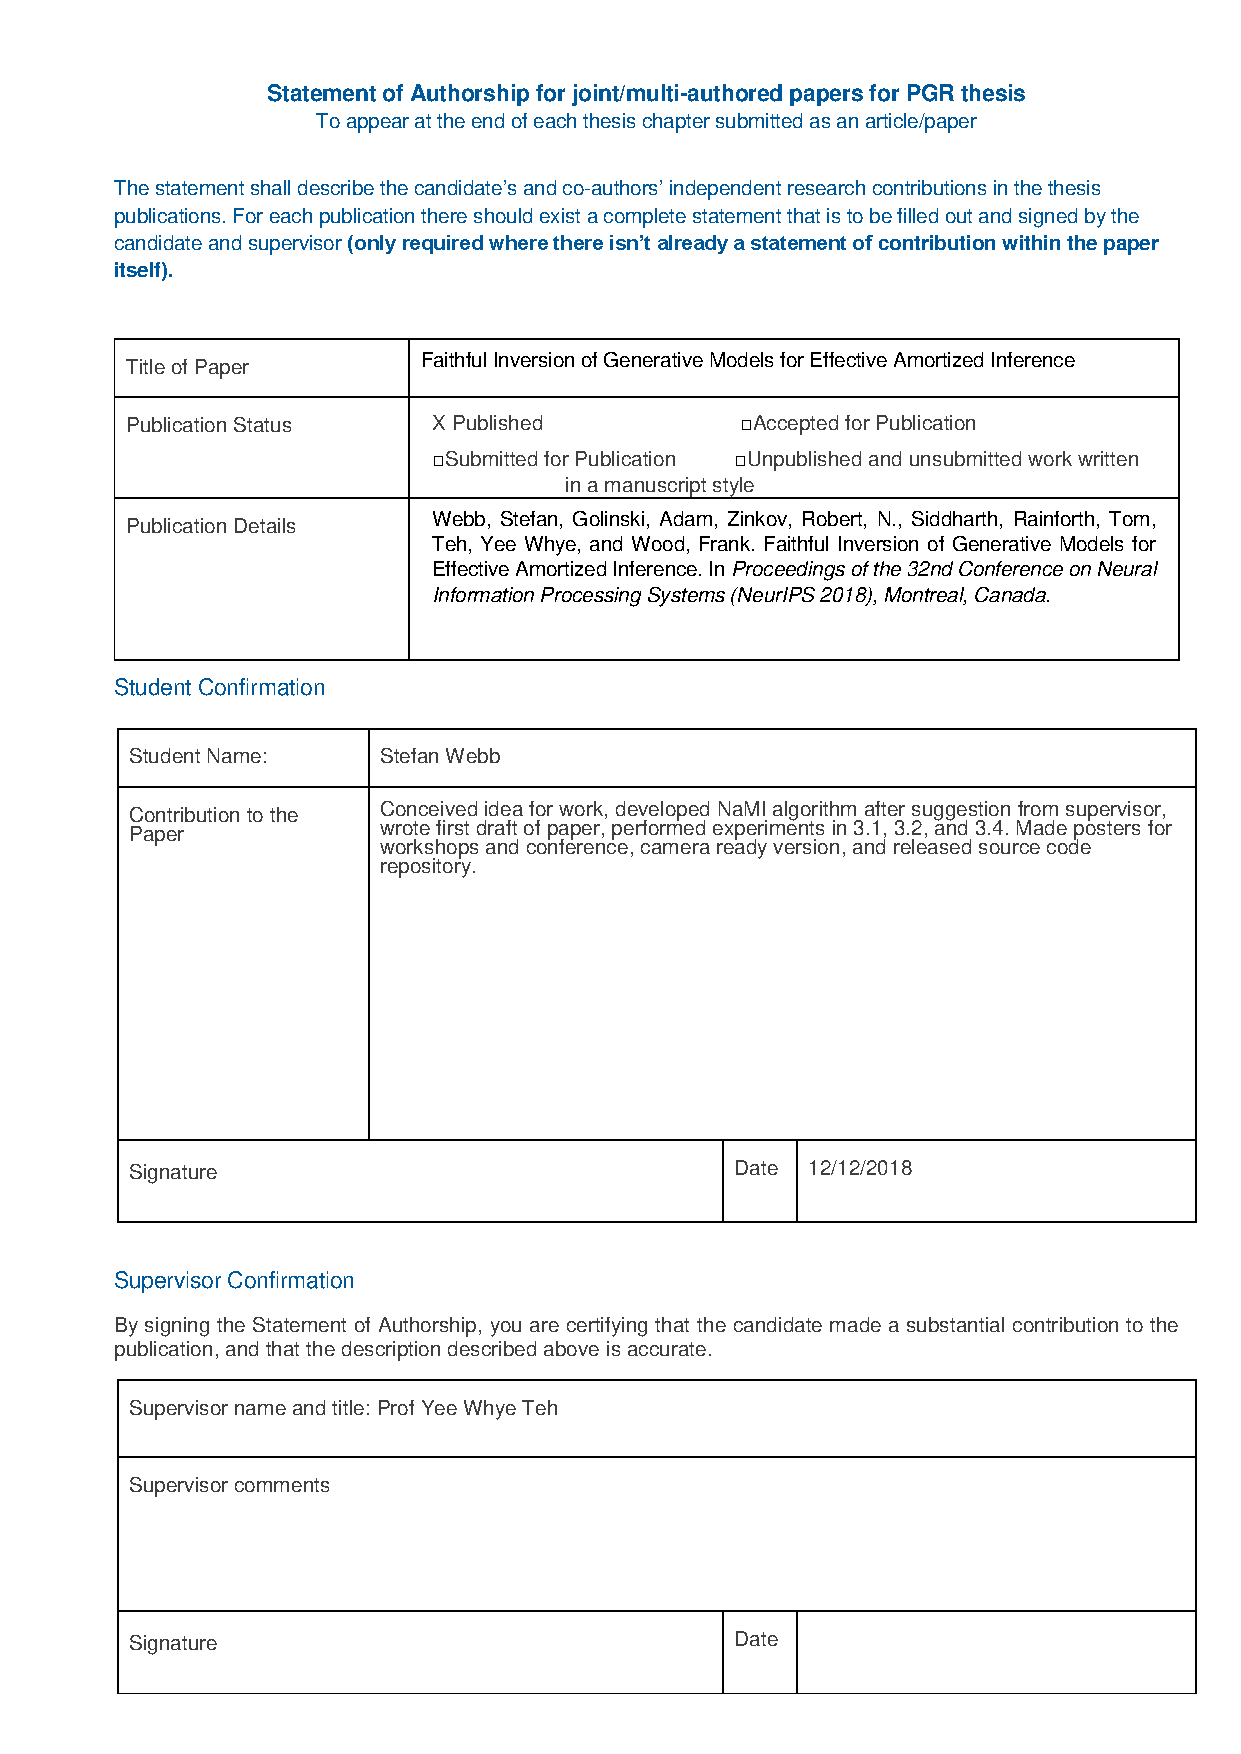
\includepdf{authorship_inverses.pdf}

\vspace{10cm}
\chapter{Distributed Bayesian Learning with SNEP and the Posterior Server}
\label{chp:posterior-server}

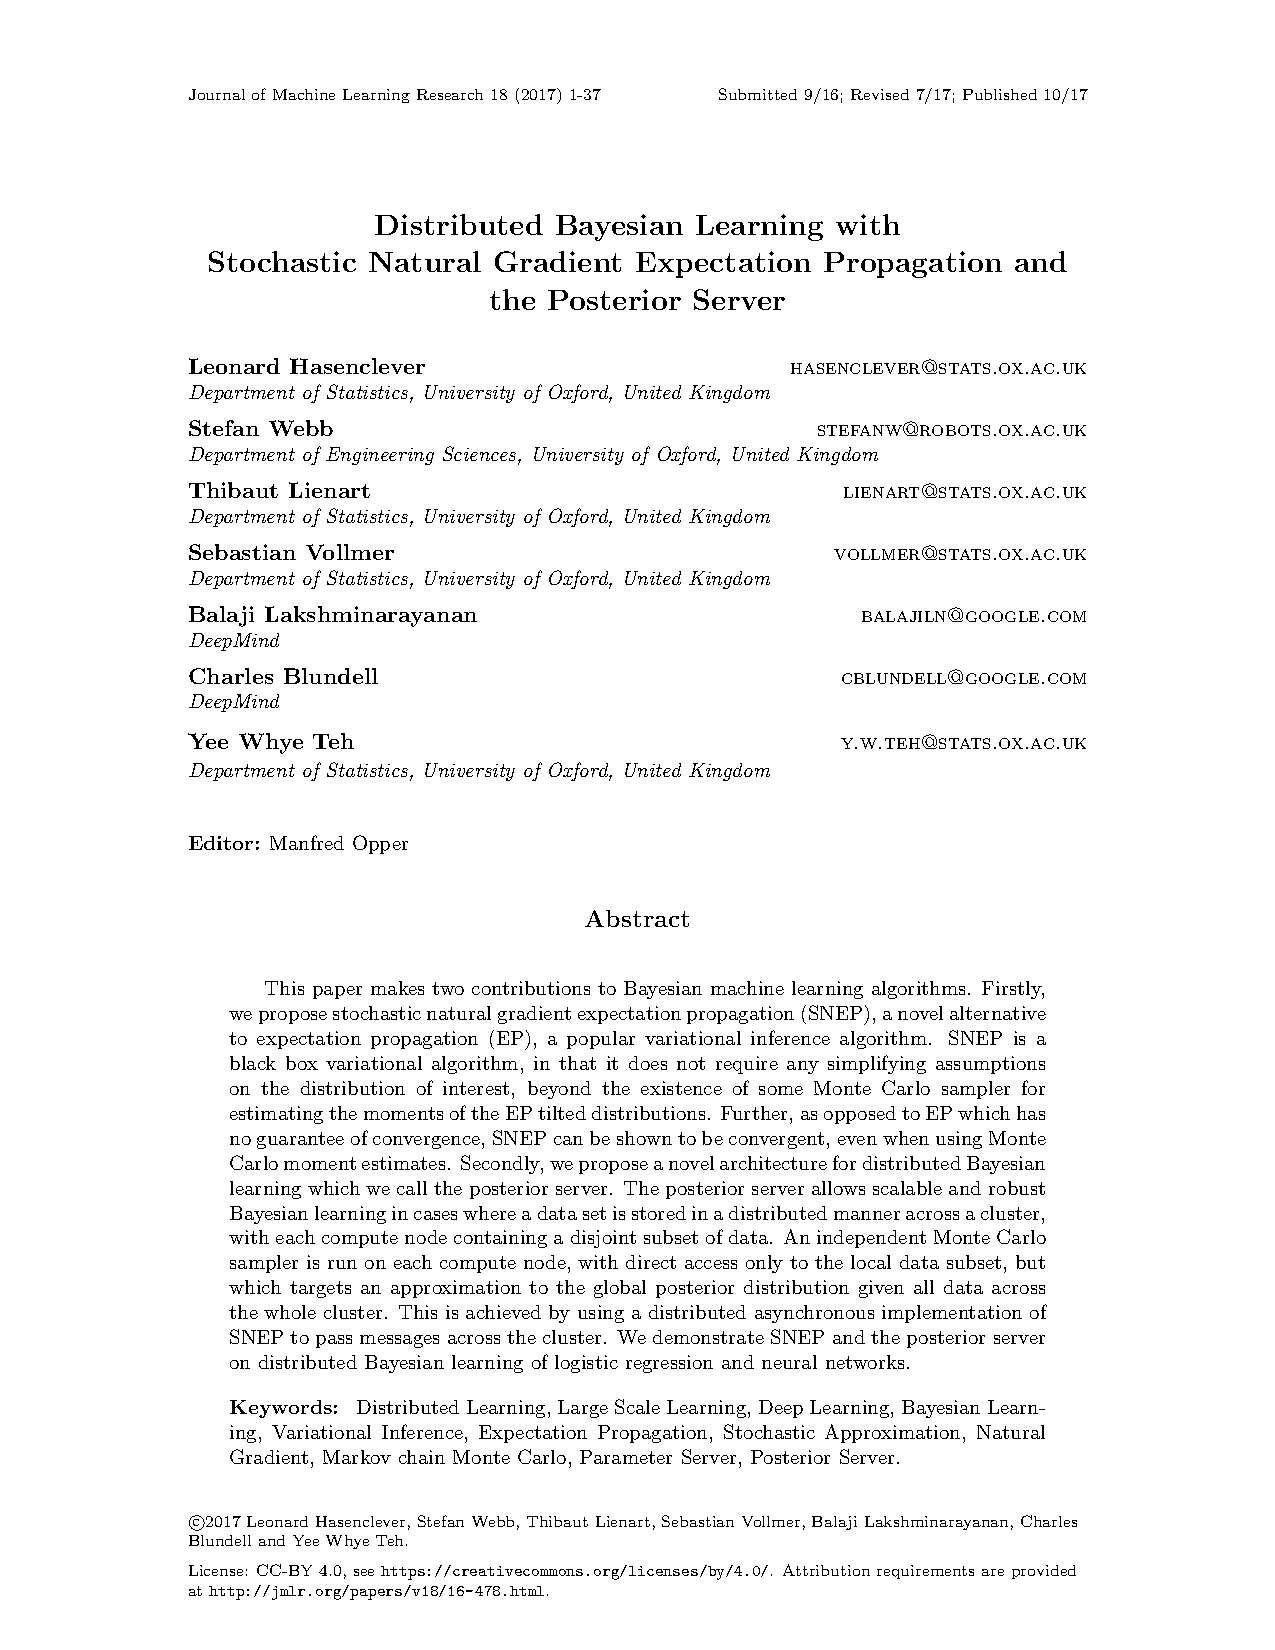
\includepdf[pages=-,noautoscale=true]{posterior_server.pdf}
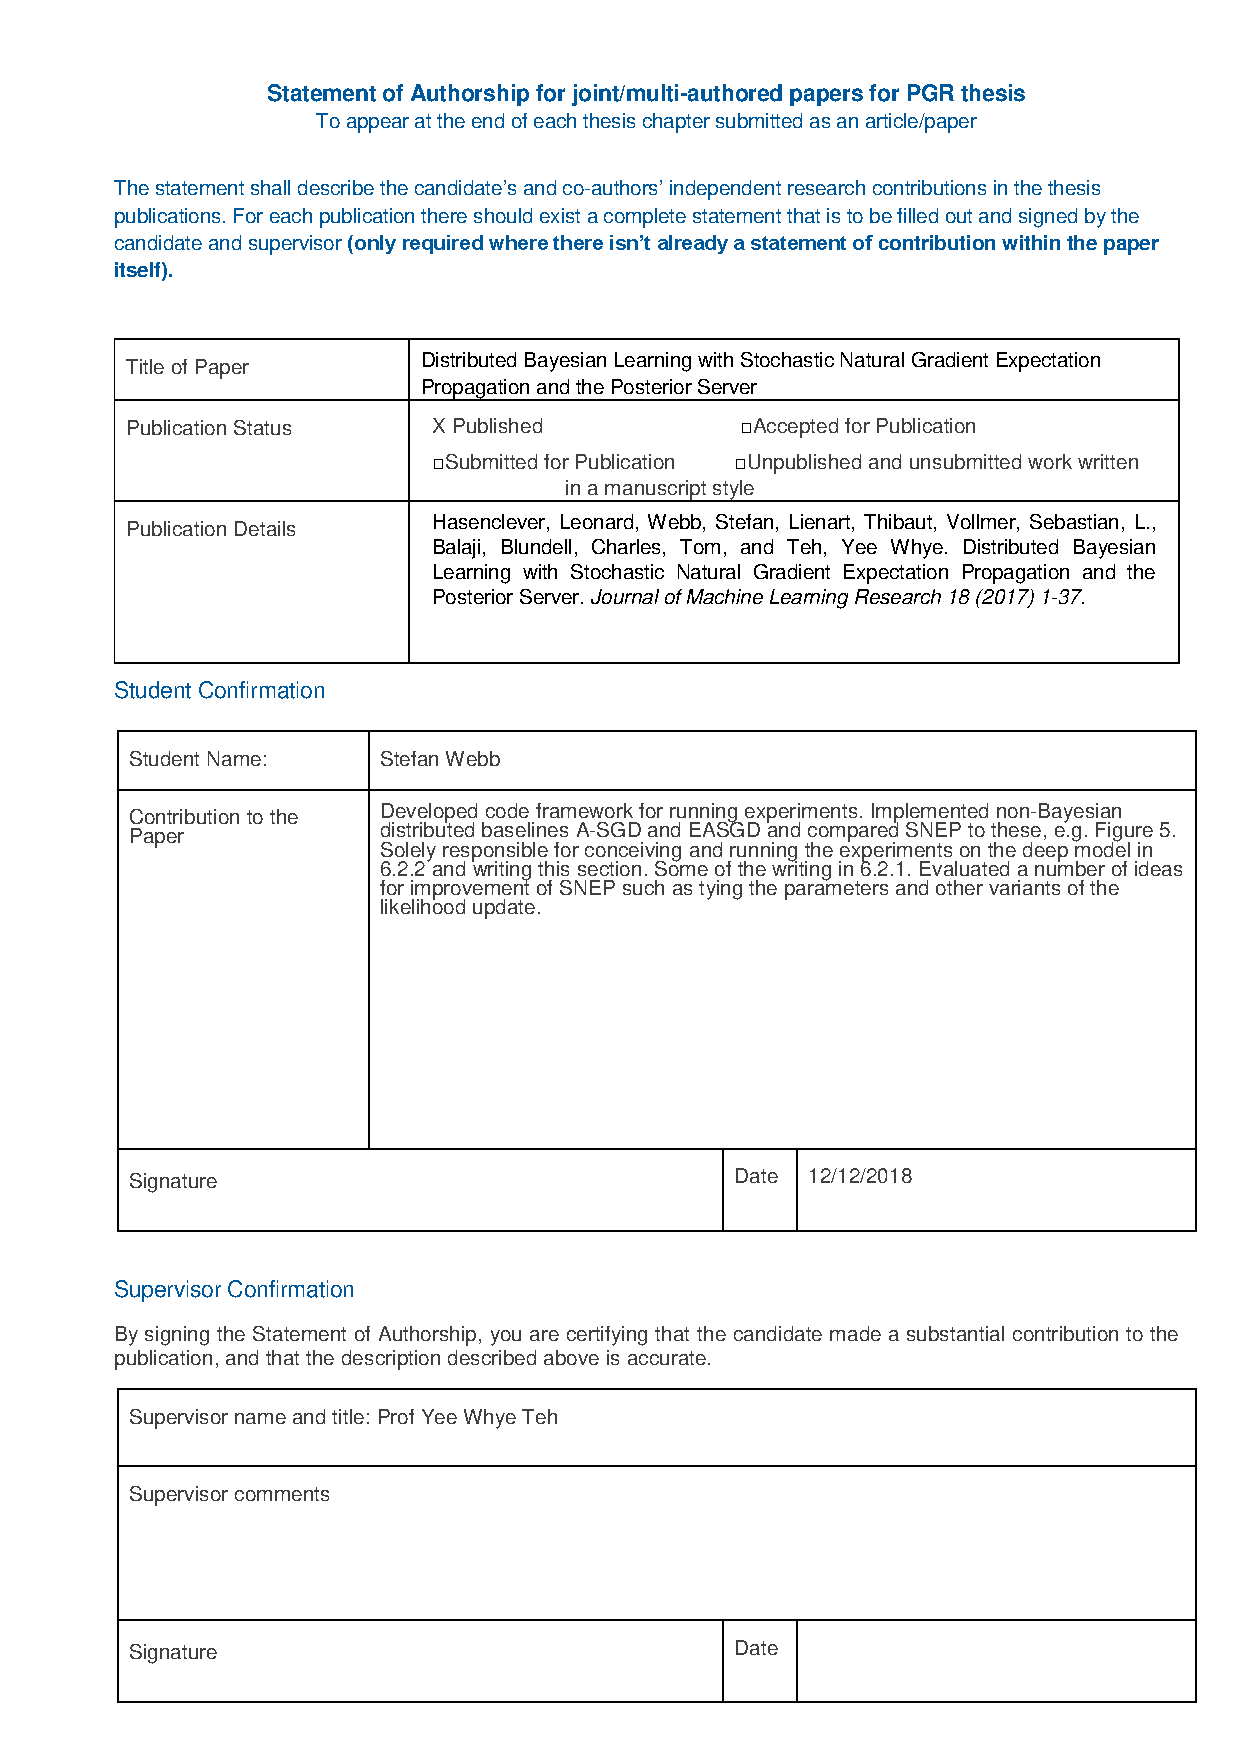
\includepdf{authorship_posterior.pdf}

\vspace{10cm}
\chapter{A Statistical Approach to Assessing Neural Network Robustness}
\label{chp:stat-verification}

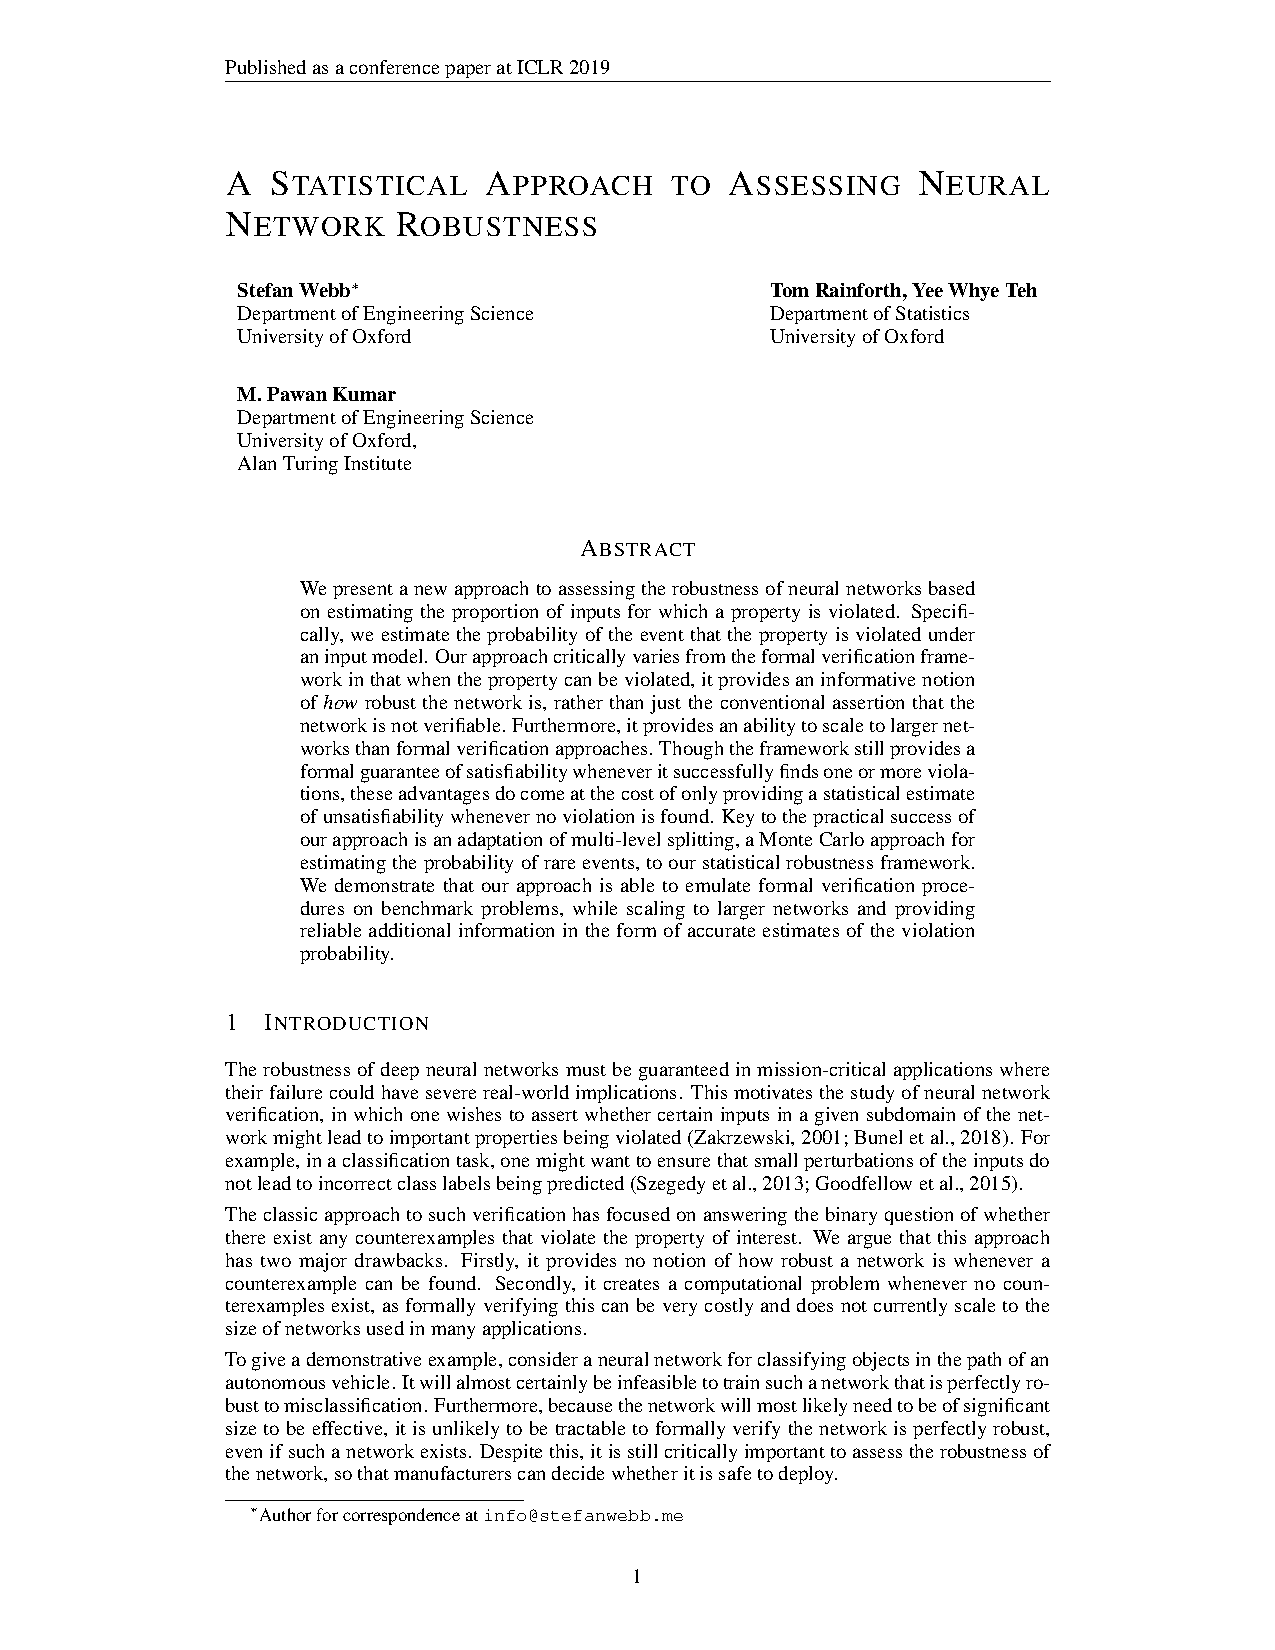
\includepdf[pages=-,noautoscale=true]{stat_verification.pdf}
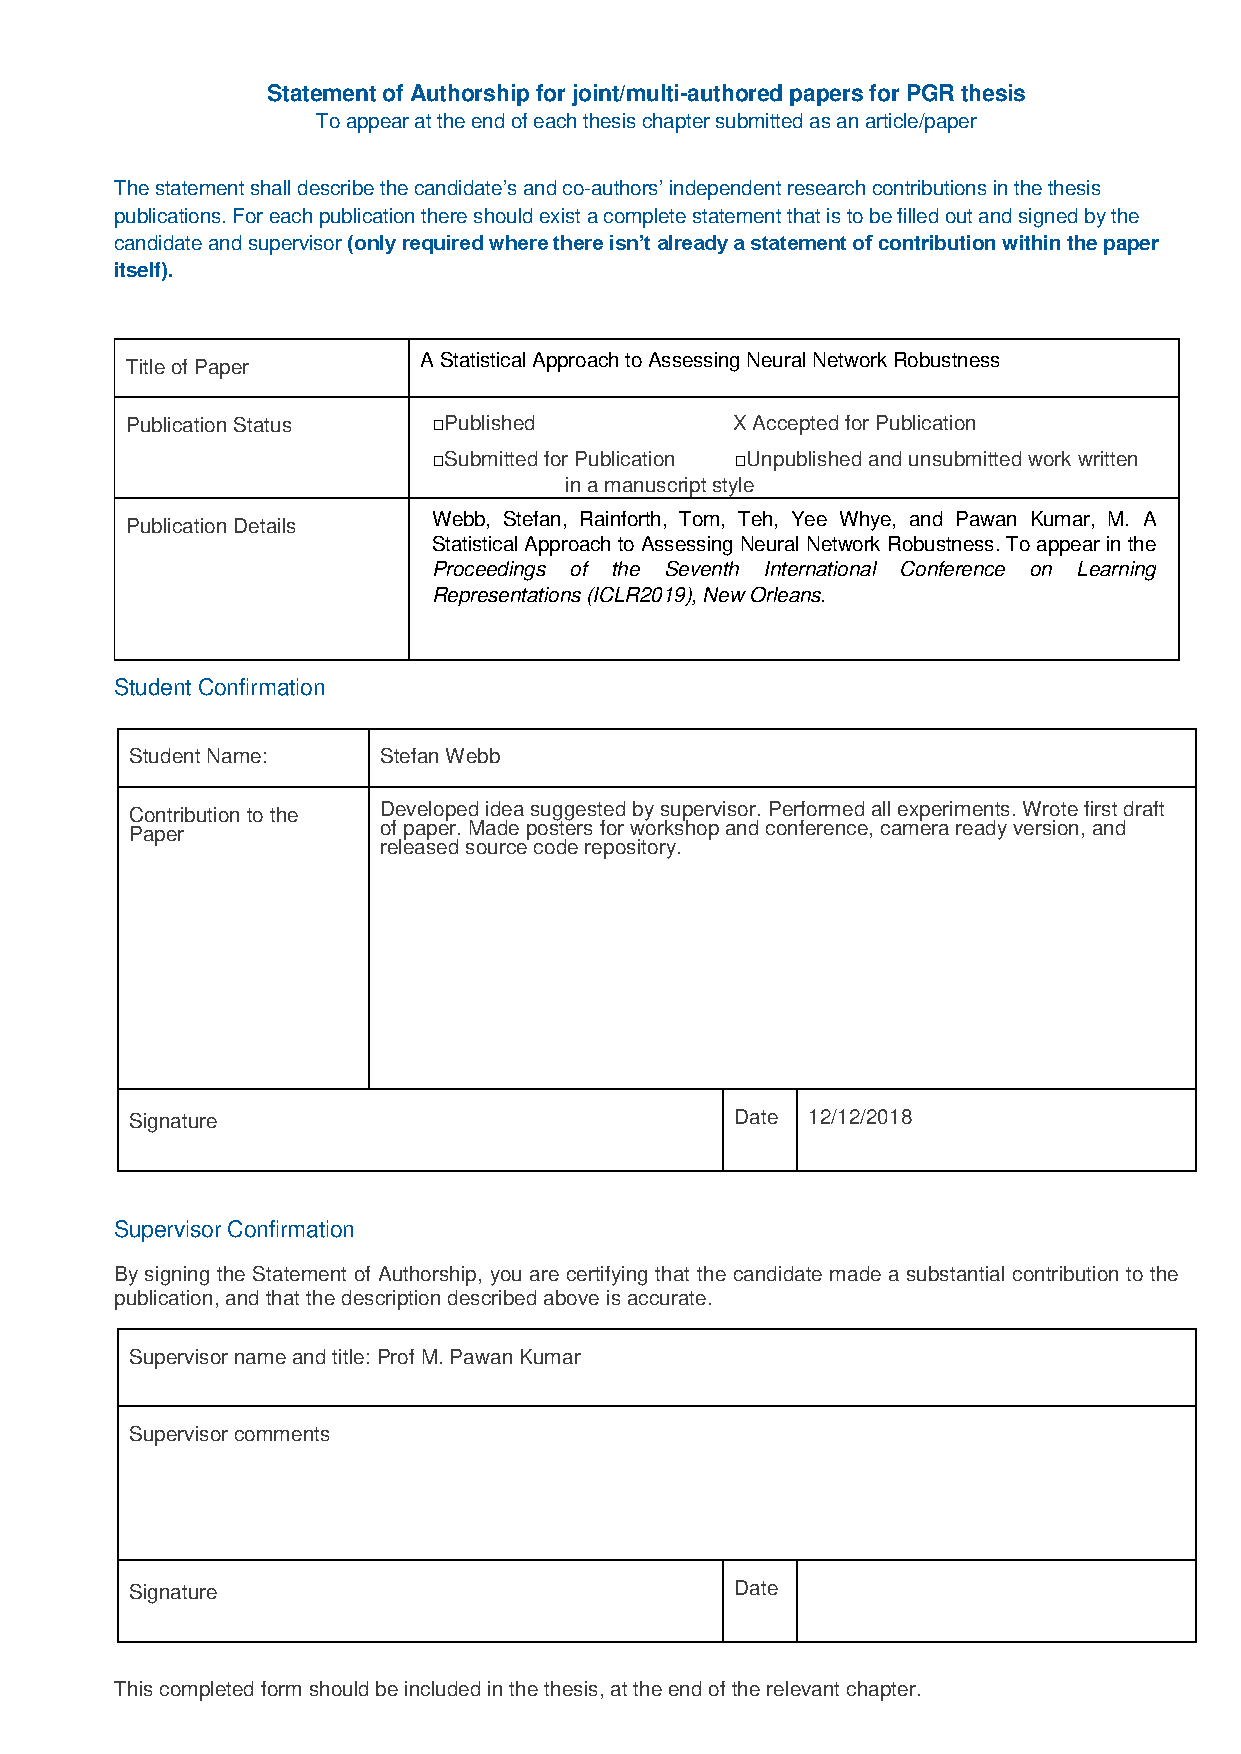
\includepdf{authorship_verification.pdf}

\chapter{Conclusions}
\label{chp:conclusions}
To recap, we have presented three original pieces of work in this thesis. The common theme has been that neural networks and deep learning are crucial for scaling Bayesian inference on generative models, and conversely that traditional Bayesian inference is important for quantifying uncertainty in NN discriminative models. In this chapter, we summarize our contributions and suggest directions for future work.

\section{Achievements}
In Ch 3, we presented the NaMI algorithm for designing the structure of inference networks and demonstrated superiority of NaMI inverses on several models. A review was given in Ch 2 of the other parts of the NaMI framework assumed in \citet{WebbEtAl2018}, namely amortized VI and NN density estimators.

In Ch 4, we presented a novel framework for distributed Bayesian learning based on a modification of the standard EP algorithm. We provided evidence that our method was able to efficiently perform distributed learning of Bayesian NNs, suffering less from the stale-gradient problem of (non-Bayesian) distributed SGD algorithms, and outperforming all other methods in learning feedforward networks with many layers of depth.

In Ch 5, we developed a novel statistical measure of neural network robustness based on a traditional inference method and demonstrated its low bias and variance, and improved scalability relative to formal verification methods.


\section{Future work}
\subsection{A statistical approach to assessing neural network robustness}
When our method is applied to adversarial properties, it produces a measure of robustness on the NN \emph{for a given image}. However, it would be desirable if we could produce a metric that measures overall robustness of the neural network, averaging over the data distribution. We believe this is an interesting and easy extension that could be accomplished by modifying the robustness metric to,
\begin{align*}
	\mathcal{I}[p,s] &\triangleq \int_{\mathcal{X}\times\mathcal{X}'}\mathbbm{1}_{\{s(\mathbf{x};\mathbf{x}')\}\ge0}p(\mathbf{x}\mid\mathbf{x}')p_\mathcal{D}(\mathbf{x}')d\mathbf{x}d\mathbf{x}',
\end{align*}
where the input model, $p(\mathbf{x},\mathbf{x}')$, can be broken up into two terms: the data distribution $p_\mathcal{D}(\cdot)$, and a uniform perturbation around the input, $p(\cdot|\mathbf{x}')$. The property function $s(\cdot)$ now becomes a function of the sampled input, $\mathbf{x}'$. Our algorithm based on AMLS would then be modified to perform the MH sampling over the modified input distribution---effectively the only change is performing approximate sampling from a distribution with double the dimension of the per-sample case.

A second extension is the investigation of improved sampling from the intermediate distributions, $\{\pi_n(\cdot)\}$. The simple Metropolis--Hastings (MH) scheme was found to be very robust and produce low bias/variance estimates in our experiments. However, it may not scale in the dimension, $D$, of larger datasets such as {\scshape ImageNet}. Even for {\scshape CIFAR}-10 (with around 4000 dimensions) the required mixing time was found to be quite large in our experiments, being around $M=2000$ steps to obtain satisfactory convergence to the target distribution. This becomes all the more important with larger models as well, for which both the constant factor of running the forward pass increases, and the number of Markov chains, $N$, that can be processed in parallel is reduced (due to limited GPU memory).

To improve the mixing time, and thus be able to reduce $M$ without introducing unacceptable bias, we propose to replace the simple MH scheme with Langevin Monte Carlo (LMC) \citep{Neal2011}. Theoretically, the computational time to reach a nearly independents sample scales as $O(D^2)$ for MH, whereas for LMC it scales as $O(D^{4/3})$. LMC can be understood as Hamiltonian Monte Carlo (HMC) with a single leapfrog step, or alternatively as a random walk that is informed by gradient information. The computational cost to reach an independent sample does scale slightly better for HMC, as $O(D^{5/4})$, although this is heavily outweighed by the increase in the constant factor due to the many more forward passes of the NN required during the leapfrog steps.

%We intend to show that LMC can produce the same results as the existing experiments but with reduced computation, judging by total wall-clock time. Then, we would like to prove that the method scales to models on {\scshape ImageNet}, which are both larger in input dimension and number of parameters.

We suggested in a previous version of \citet{webb2018statistical} that the adversarial samples produced by our algorithm may be of interest for adversarial training. However, it takes several minutes in typical usage to pass through all the levels to obtain samples from the final $\pi_K$. While it may not, therefore, be practical to \emph{directly} use the samples from our algorithm for robustness training, we believe that a robust training method could be formed from the fundamental idea of our work, of sampling adversarial, or near-adversarial, samples by MCMC methods. Let us elaborate.

Many robust training methods can be understood as approximations to the following variant of empirical risk minimization \citep{madry2017towards, tramer2017ensemble},
\begin{align*}
	f^* &= \text{argmax}_{f\in\mathcal{F}}\mathbb{E}_{(\mathbf{x},y^*)\sim\mathcal{D}}\left[\max_{||\mathbf{x}'-\mathbf{x}||_\infty\le\epsilon}s(\mathbf{x}';f,\mathbf{x},y^*)\right],
\end{align*}
where $y^*$ is the true class label. For instance, the iterative fast gradient-sign method (I-FGSM) \citep{goodfellow2014explaining} approximates the inner max term by starting from $x$ and taking $k$ steps of size $\alpha=\epsilon/k$ in the direction of the sign of the gradient of the property function, clipping where necessary to keep within the $l_\infty$ $\epsilon$-ball and the valid range of pixels. In another method \citep{kolter2017provable, wong2018explaining}, a convex outer bound, $E\subseteq\{\mathbf{x}'\mid s(\mathbf{x}';f,\mathbf{x},y^*)\ge0\}$ is produced and the max performed over $\mathbf{x}'\in E$.

As pointed out in \citep{tramer2017ensemble}, if the approximation to the max term is poor, that is,
\begin{align*}
	s(\mathbf{x}^*;f,\mathbf{x},y^*) &\ll  \max_{||\mathbf{x}'-\mathbf{x}||_\infty\le\epsilon}s(\mathbf{x}';f,\mathbf{x},y^*)
\end{align*}
where $\mathbf{x}^*$ is the sample produced by the approximation method, then the adversarial training degrades the quality of adversarial samples generated by the model, which then degrades the quality of subsequent adversarial training. The result of this is that the model reaches an equilibrium during training where it can effectively defend against white-box but not black-box attacks, those where the adversarial samples are transferred from another model.

The authors suggest a new method for adversarial training in which they decouple adversarial training from adversarial generation, and use samples from an ensemble of additional source models that are held constant during the adversarial training of the target model (adding a small amount of random noise to each). In this way, the adversarial training does not influence the generation of samples used for the training. This relies on the heuristic that adversarial examples often transfer across models. However, it does seem unsatisfactory in that we are no longer directly solving the objective, and it may not be the case that examples do transfer across all architectures or that the transferable examples are representative of all adversarial examples on the model.

We propose to modify the objective to,
\begin{align*}
	f^* &= \text{argmax}_{f\in\mathcal{F}}\mathbb{E}_{(\mathbf{x},y^*)\sim\mathcal{D}}\left[\mathbb{E}_{\mathbf{x}'\sim p(\cdot|\mathbf{x})}\left[s(\mathbf{x}';f,\mathbf{x},y^*)\right]\right],
\end{align*}
where, for instance, $p(\mathbf{x}'|\mathbf{x})\propto\exp(s(\cdot|\mathbf{x}))\mathbbm{1}_{\{||\mathbf{x}'-\mathbf{x}||_\infty\le\epsilon\}}$. We can draw approximate samples from $p$ by LMC.

This method has several advantages. Firstly, we can produce multiple proposal samples per data point directly from the model in question, as opposed to only a single proposal sample from the model like in the I-FGSM method and that of \citet{kolter2017provable}, or a number of samples per data point from surrogate models, like \citet{tramer2017ensemble}. Also, by the reliability of the sampling process, we can ensure that the proposals are diverse and are  adversarial or near-adversarial, thus avoiding the poor equilibrium discussed before. As argued in \citet{webb2018statistical}, in many cases it makes more sense to define robustness in terms of the prevalence of adversarial examples in the vicinity of a data point rather than the distance to the nearest one, and for this reason we would expect a training algorithm that trains on multiple and diverse adversarial examples per data point to be more effective in reducing our measure of robustness. Our proposed method is also fast, requiring only a few extra gradient steps per minibatch over the I-FGSM.

%We would like to compare our method to other robust training methods like I-FGSM and \citet{kolter2017provable} measured by both our novel robustness metric and by the fraction of samples that are provably robust to perturbations within a given radius, and show that it is more efficient in quickly increasing robustness, while obtaining a better solution at convergence.

\subsection{Faithful inverses for effective amortized inference}
A very worthy outstanding challenge of Bayesian statistics is that of producing \emph{universal automated inference}. Such a hypothesized inference scheme is said to be \emph{universal} in that it would be applicable to higher-order probabilistic programs, those with recursion, other stochastic control flow mechanisms, and high-order functions, and, \emph{automated} in that it would not require any intervention by the user after having specified the model and the query of interest in the details of how inference is applied.

A universal inference scheme based on amortized VI and the Anglican PPL \citep{wood2014new} was attempted in \citet{LeEtAl2016}. Their method used particle-based inference with a data driven proposal to learn to perform inference in a universal PPL. As noted by the authors, it suffered from two shortcomings. Firstly, the method did not perform model learning, and as discovered in the experiments on CAPCHA solving, it is difficult to program a correct model ab initio. Secondly, the inference network conditioned on all previous random choices, not only the relevant ones (from the PGM perspective of \citet{WebbEtAl2018}). As demonstrated in our work, this slows learning considerably and leads convergence to a worse solution.

We believe this important work is based on the most promising approach for universal automated inference, that of amortized VI, and that it can be further developed to overcome the hurdles the authors discovered. Firstly, new learning algorithms have been developed that would be suitable for probabilistic programs, with their seqential nature. For instance, filtering variational objectives, in a sense, can differentiate through particle-based inference algorithms in order to perform model learning \citep{MaddisonEtAl2017, LeEtAl2017, NaessethEtAl2017}. Secondly, the development of the NaMI algorithm provides an intelligent way to automate the design of the structure of the inference network. Currently, either the modeler must design the inference network by hand, or use an unstructured fully connected one (e.g., see the existing autoguides of Pyro \citep{bingham2018pyro}).

We intend to integrate the NaMI algorithm into the Pyro PPL for designing the structure of an inference network, and use heuristics for designing the parametrization based on normalizing flows. PPLs provide the necessary abstractions, in this case \emph{poutines}, to manipulate a representation of the model in order to operate the NaMI algorithm and choose an appropriate factorization.

At first, we intend to demonstrate inference compilation on models with a fixed structure, such as traditional BNs. We believe the importance of a structured inference network increases in the scale of the model---an heuristic approach diverges more from the posterior as the number of variables increases, and a fully connected approach suffers the curse of dimensionality. Some traditional factor graph BNs, for example, those used for medical diagnosis, have thousands of variables, and would be suitable for this experimentation. Performing fast inference in these models is very important in industry. %We would then like to attempt to automate the design of inference networks for models with limited forms of dynamic structure.

Some challenges in automating the design of inference networks include automating the design of the NN encoder and decoder architectures and selection of hyperparameters like the learning rates. It is likely that meta-learning approaches are necessary, which learn from their past successes and failures and are able to generalize to novel scenarios.

%\startappendices
%\input{appendices/appendices}

\clearpage
\renewcommand{\chapterheadstartvskip}{\vspace*{-30pt}}
\bibliography{dphil}

\end{document} 

